\documentclass[hidelinks,11pt,dvipsnames]{article}
% xcolor commonly causes option clashes, this fixes that
\PassOptionsToPackage{dvipsnames,table}{xcolor}
\usepackage[tmargin=1in, bmargin=1in, lmargin=0.8in, rmargin=1in]{geometry}

%%%%%%%%%%%%%%%%%%%%%%%%%%%%%%%%%%%%%%%%%%%%%%%%%%%%%%%%%%%%%%%%%%%%
%%% For inkscape-figures
%%% Assumes the following directory structure:
%%% master.tex
%%% figures/
%%%     figure1.pdf_tex
%%%     figure1.svg
%%%     figure1.pdf
%%%%%%%%%%%%%%%%%%%%%%%%%%%%%%%%%%%%%%%%%%%%%%%%%%%%%%%%%%%%%%%%%%%%
%\usepackage{import}
\usepackage{pdfpages}
\usepackage{transparent}

\newcommand{\incfig}[2][1]{%
    \def\svgwidth{#1\columnwidth}
    \import{./figures/}{#2.pdf_tex}
}

\pdfsuppresswarningpagegroup=1

% enable synctex for inverse search, whatever synctex is
\synctex=1
\usepackage{float,macrosabound,homework,theorem-env}
\usepackage{microtype}


% font stuff
\usepackage{sectsty}
\allsectionsfont{\sffamily}
\linespread{1.1}

% bibtex stuff
\usepackage[backend=biber,style=alphabetic,sorting=anyt]{biblatex}
\addbibresource{main.bib}

% colored text shortcuts
\newcommand{\blue}[1]{\color{MidnightBlue}{#1}}
\newcommand{\red}[1]{\textcolor{Mahogany}{#1}}
\newcommand{\green}[1]{\textcolor{ForestGreen}{#1}}


% use mathptmx pkg while using default mathcal font
\DeclareMathAlphabet{\mathcal}{OMS}{cmsy}{m}{n}

% fixes the positioning of subscripts in $$ $$
\renewcommand{\det}{\operatorname{det}}

\usetikzlibrary{positioning, arrows.meta}
\newcommand{\here}[2]{\tikz[remember picture]{\node[inner sep=0](#2){#1}}}

%%%%%%%%%%%%%%%%%%%%%%%%%%%%%%%%%%%%%%%%%%%%%%%%%%%%%%%%%%%%%%%%%%%%%
%%% Entry Counter
%%%%%%%%%%%%%%%%%%%%%%%%%%%%%%%%%%%%%%%%%%%%%%%%%%%%%%%%%%%%%%%%%%%%%
\newcounter{entry-counter}
\newcommand{\entry}[1]
{
	\addtocounter{entry-counter}{1}
    \tchap{Entry \arabic{entry-counter}}
	%\addcontentsline{toc}{section}{Entry \arabic{entry-counter}: #1}
	\vspace{-1.5em}
    \begin{center}
		\small \emph{Written: #1}
    \end{center}
}

\usepackage{titling}
\renewcommand\maketitlehooka{\null\mbox{}\vfill}
\renewcommand\maketitlehookd{\vfill\null}


\usepackage{caption}
\usepackage{tikz}
\usetikzlibrary{positioning,calc,intersections,through,backgrounds, shapes.geometric, decorations.markings,arrows}

\def\sset{\subseteq}
\def\iso{\cong}
\def\gend#1{\langle #1\rangle}

\newcommand{\rightoverleftarrow}{%
  \mathrel{\vcenter{\mathsurround0pt
    \ialign{##\crcr
      \noalign{\nointerlineskip}$\longrightarrow$\crcr
      \noalign{\nointerlineskip}$\longleftarrow$\crcr
    }%
  }}%
}

\newcommand\makesphere{} % just for safety
\def\makesphere(#1)(#2)[#3][#4]{%
  % Synopsis
  % \makesphere[draw options](center)(initial angle:final angle:radius)
  \shade[ball color = #3, opacity = #4] #1 circle (#2);
  \draw #1 circle (#2);
  \draw ($#1 - (#2, 0)$) arc (180:360:#2 and 3*#2/10);
  \draw[dashed] ($#1 + (#2, 0)$) arc (0:180:#2 and 3*#2/10);
}
% same thing as makesphere but places white background behind
\newcommand\altmakesphere{} % just for safety
\def\altmakesphere(#1)(#2)(#3)[#4][#5]{%
  % Synopsis
  % \makesphere[draw options](center)(initial angle:final angle:radius)
  \draw [fill=white!30] #1 circle (#2);
  \shade[ball color = #4, opacity = #5] #1 circle (#2);
  \draw #1 circle (#2);
  \draw ($#1 - (#2, 0)$) arc (180:360:#2 and 3*#2/10);
  \draw[dashed] ($#1 + (#2, 0)$) arc (0:180:#2 and 3*#2/10);
  \node at #1 {#3};
}

\begin{document}
\pagestyle{empty}
	\LARGE
\begin{center}
	Algebraic Topology Homework 4 \\
	\Large
	Isaac Martin \\
    Last compiled \today
\end{center}
\normalsize
\vspace{-4mm}
\hru

\tchap{Problems from 1.2}
\begin{homework}[e]
  \prob[\textsc{Exercise 1.9}] In the surface $M_g$ of genus $g$, le $C$ be a circle that separates $M_g$ into two compact subsurfaces $M'_h$ and $M'_k$ obtained from the closed surfaces $M_h$ and the $M_k$ by deleting an open disk from each. Show that $M'_h$ does not retract onto its boundary circle $C,$ and hence $M_g$ does not retract onto $C$. [Hint: abelianize $\pi_1$.] But show that $M_g$ does retract onto the nonseparating circle $C'$ in the figure.
  \begin{prf}
    The surface $M_h$ is constructed f rom $2h$ one-cells and $1$ two-cell. Deleting an open disk from $M_h$ is equivalent to deleting an open disk from the interior of the two-cell prior to identification, but this space is readily seen to deformation retract onto its boundary (see figure \ref{fig:prob9.1}).
    \begin{center}
      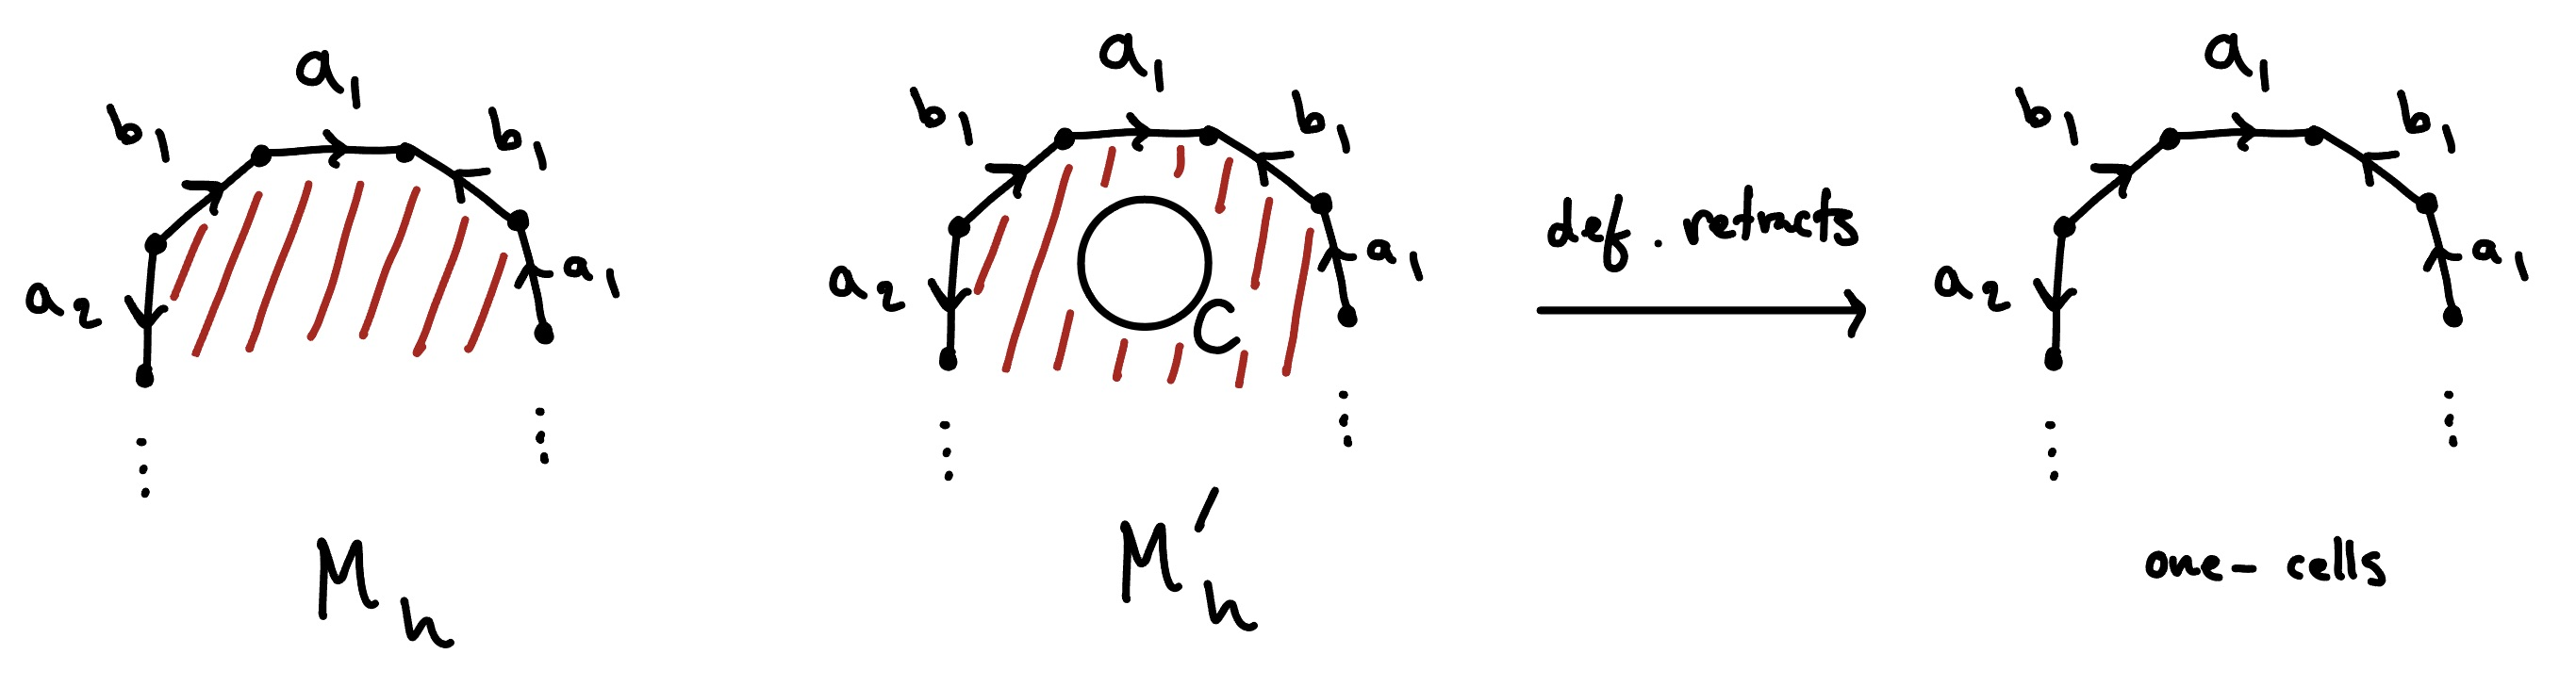
\includegraphics[width=10cm]{figures/hwk4-fig0.png}
      \captionof{figure}{$M_h'$ deformation retracts to one-skeleton}
      \label{fig:prob9.1}
    \end{center}
    Deformation retractions induce isomorphisms, so $\pi_1(M_h') \cong \pi_1(M_{h,0}),$ which is simply a free product on $2h$ generators. The Abelianization of $\pi_1(M_h')$ is therefore $\bZ^{\oplus 2h}$, isomorphic to the Abelianization of $\pi_1(M_h)$.

    Suppose we did have a retraction $r:M'_h \to C$. The inclusion $\iota:C\to M_h'$ would then induce an injection $\iota_*:\pi_1(C) \to \pi_1(M_h')$. As $M_h$ is obtained from $M_h'$ by attaching a $2$-cell with boundary $C$, by Proposition 1.26 (a) the inclusion $M_h' \hookrightarrow M_h$ induces a surjection $\varphi:\pi_1(M_h')\to \pi_1(M_h)$ whose kernel is comprised of loops around $C$: $\iota_*(\pi_1(C))$. We would then have
    \begin{align*}
      \pi_1(M'_h)/\iota_*(\pi_1(C)) \cong \pi_1(M_h).
    \end{align*}
    However, taking the Abelianization of the above, we obtain
    \begin{align*}
      \bZ^{\oplus 2h}/n\bZ \cong \bZ^{\oplus 2h},
    \end{align*}
    for some $0 \neq n \in \bZ$ (we write $n\bZ$ rather than $\bZ$ for the Abelianization of $\iota_*(\pi_1(\bZ))$ since we have not described precisely what the embedding actually is, only that it is an embedding). This is impossible, since the group on the left is either a free $\bZ$-module of rank $2h - 1$ or has torsion, while the group on the right is a free $\bZ$-module of rank $2h$. We therefore cannot have a retraction $r:M'_h \to C$.

    We now show that $M_g$ does retract onto $C'$. Consider first the case $g = 1$, $M_1 = S_1\times S_1$. To keep notation consistent, we can let $C'$ be the first component of the product so that $M_1 = C'\times S^1$. Let $r:C'\times S^1\to C'$ be the projection onto the first coordinate, i.e. $r(\{s_0\}\times S^1) = s_0$ for all $s_0 \in C'$. This map fixes $C'$ and is continuous since for each $U \subseteq U$ we have $r^{-1}(U) = U\times S^1$, which is open in product topology by definition. Hence $r$ is a retraction of $M_1$ onto $C'$.

    To extend this argument to arbitrary $g$, consider again the standard $1$-skeleton of $M_g$ $X^1 = \bigvee_{i=1}^g S^1_{a_i}\vee \S^1_{b_i}$ and let $\varphi:S^1\to X^1$ be the attaching map. Collapsing $\bigvee_{i=2}^g S^1_{a_i}\vee \S^1_{b_i}$ to the base point gives us a quotient $g:M_g\to M_1$. The composition $r\circ q$ is then a retraction of $M_g$ onto $C'$.
  \end{prf}
  \prob[\textsc{Exercise 1.10}] Consider two arcs $\alpha$ and $\beta$ embedded in $D^2 \times I$ as shown in the figure. The loop $\gamma$ is obviously nullhomotopic in $D^2\times I$ , but show that there is no nullhomotopy of $\gamma$ in the complement of $\alpha \cup \beta$.
  \begin{prf}
    The key here is to realize that the knot formed by $\alpha$ and $\beta$ can be unraveled to obtain a homotopy equivalence between our space $D^2\times I - (\alpha \cup \beta)$ and the cylinder with two parallel lines removed. We move the endpoints of $\alpha$ and $\beta$, carrying $\gamma$ throughout the process.
    \begin{center}
      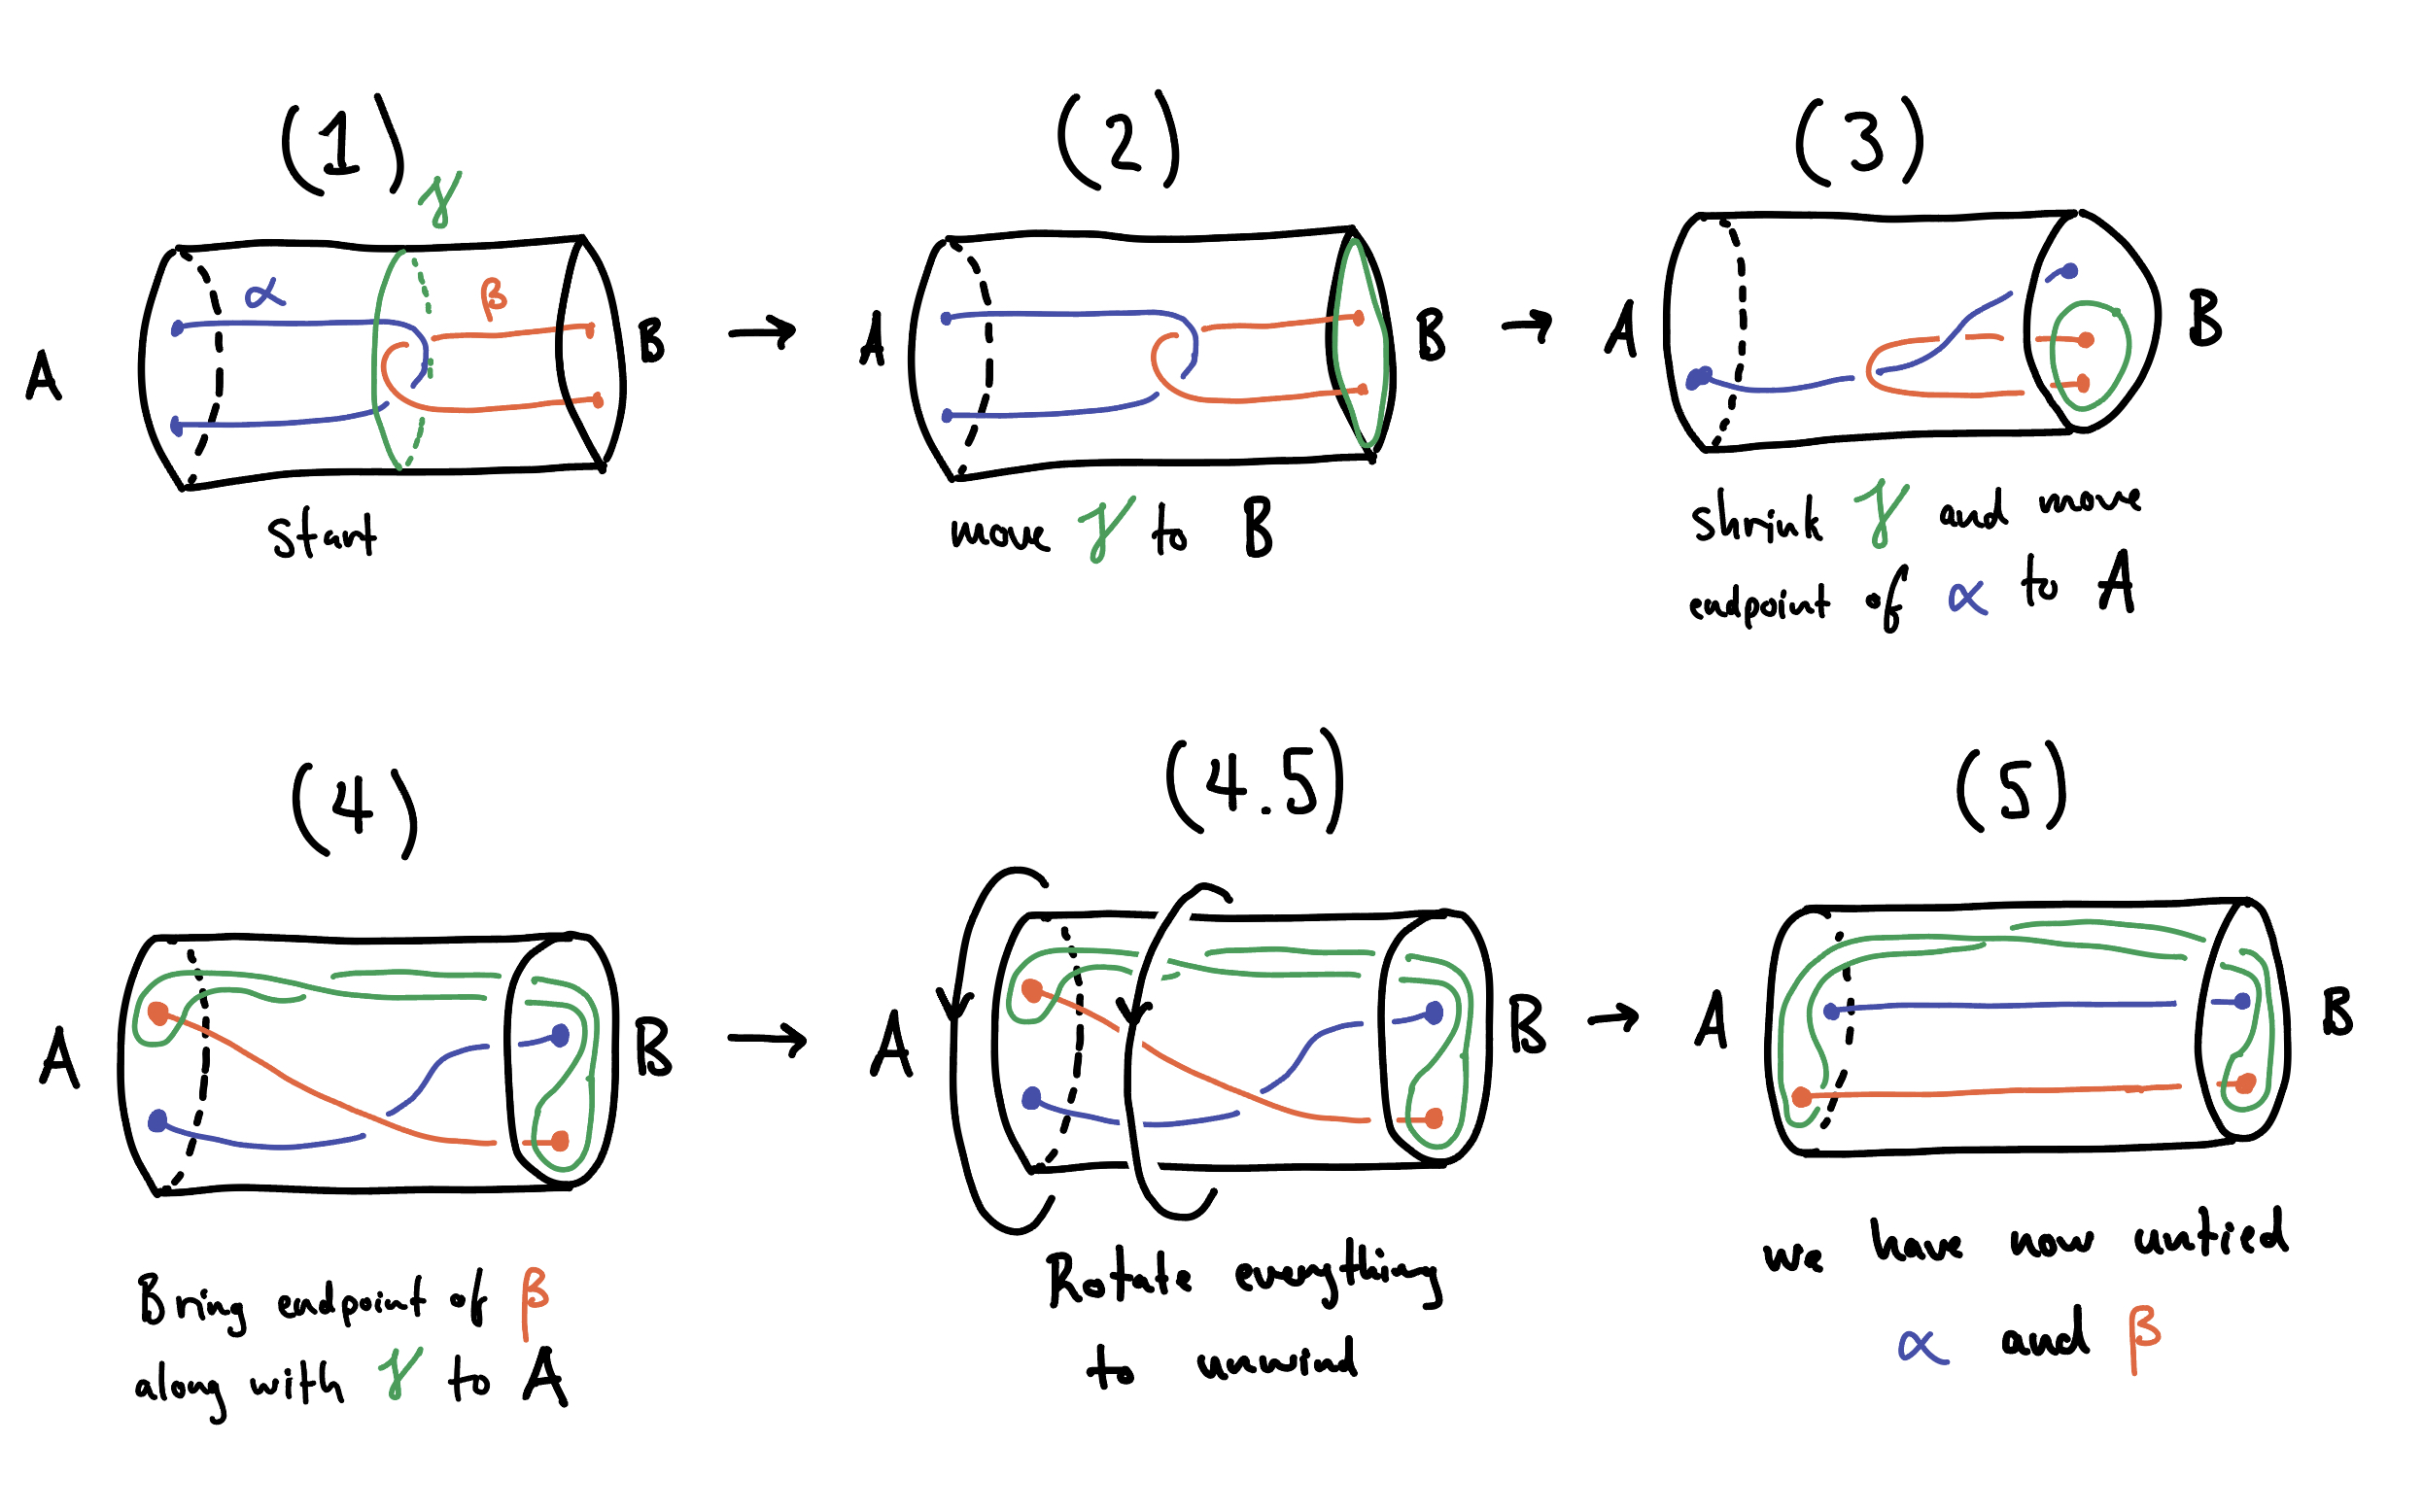
\includegraphics[width=15cm]{figures/hwk4-fig1.jpg}
      \captionof{figure}{Unraveling $\alpha$ and $\beta$}
      \label{fig:prob10.1}
    \end{center}
    The cylinder with two lines removed deformation retracts to $D^2$ with two points removed, which we also label $\alpha$ and $\beta$. Call this new space $Y$.
    \begin{center}
      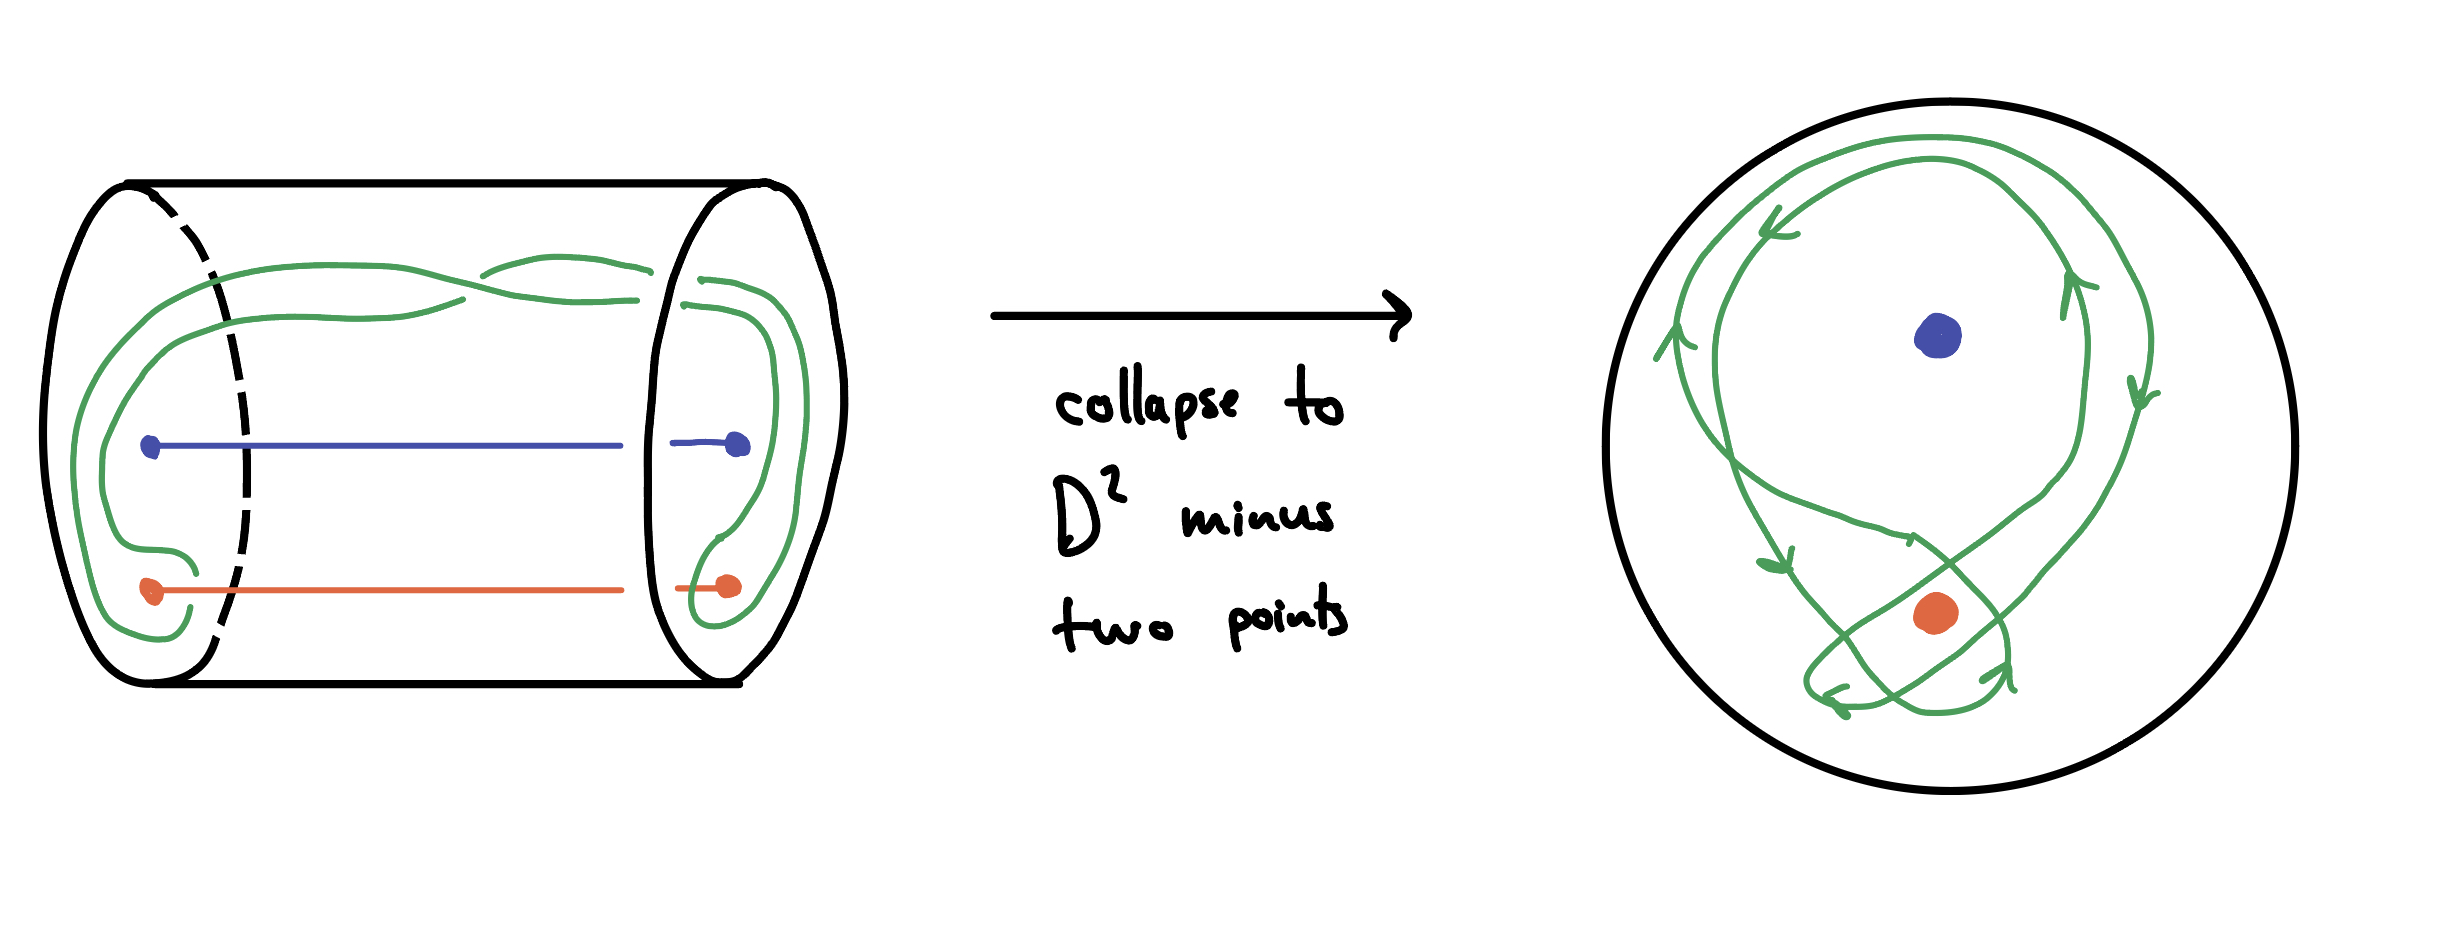
\includegraphics[width=12cm]{figures/hwk4-fig2.jpg}
      \captionof{figure}{Deformation retract of (5) onto $Y = D^2 - \{\alpha,\beta\}$}
      \label{fig:prob10.2}
    \end{center}
    The space $Y$ deformation retracts onto the wedge of two circles, the only question is what happens to the path $\gamma$ during this process. Figure (\ref{fig:prob10.3}) illustrates a homotopy of $\gamma$ which makes its image under the deformation retract of $Y$ to $S^1\vee S^1$ more clear.
    \begin{center}
      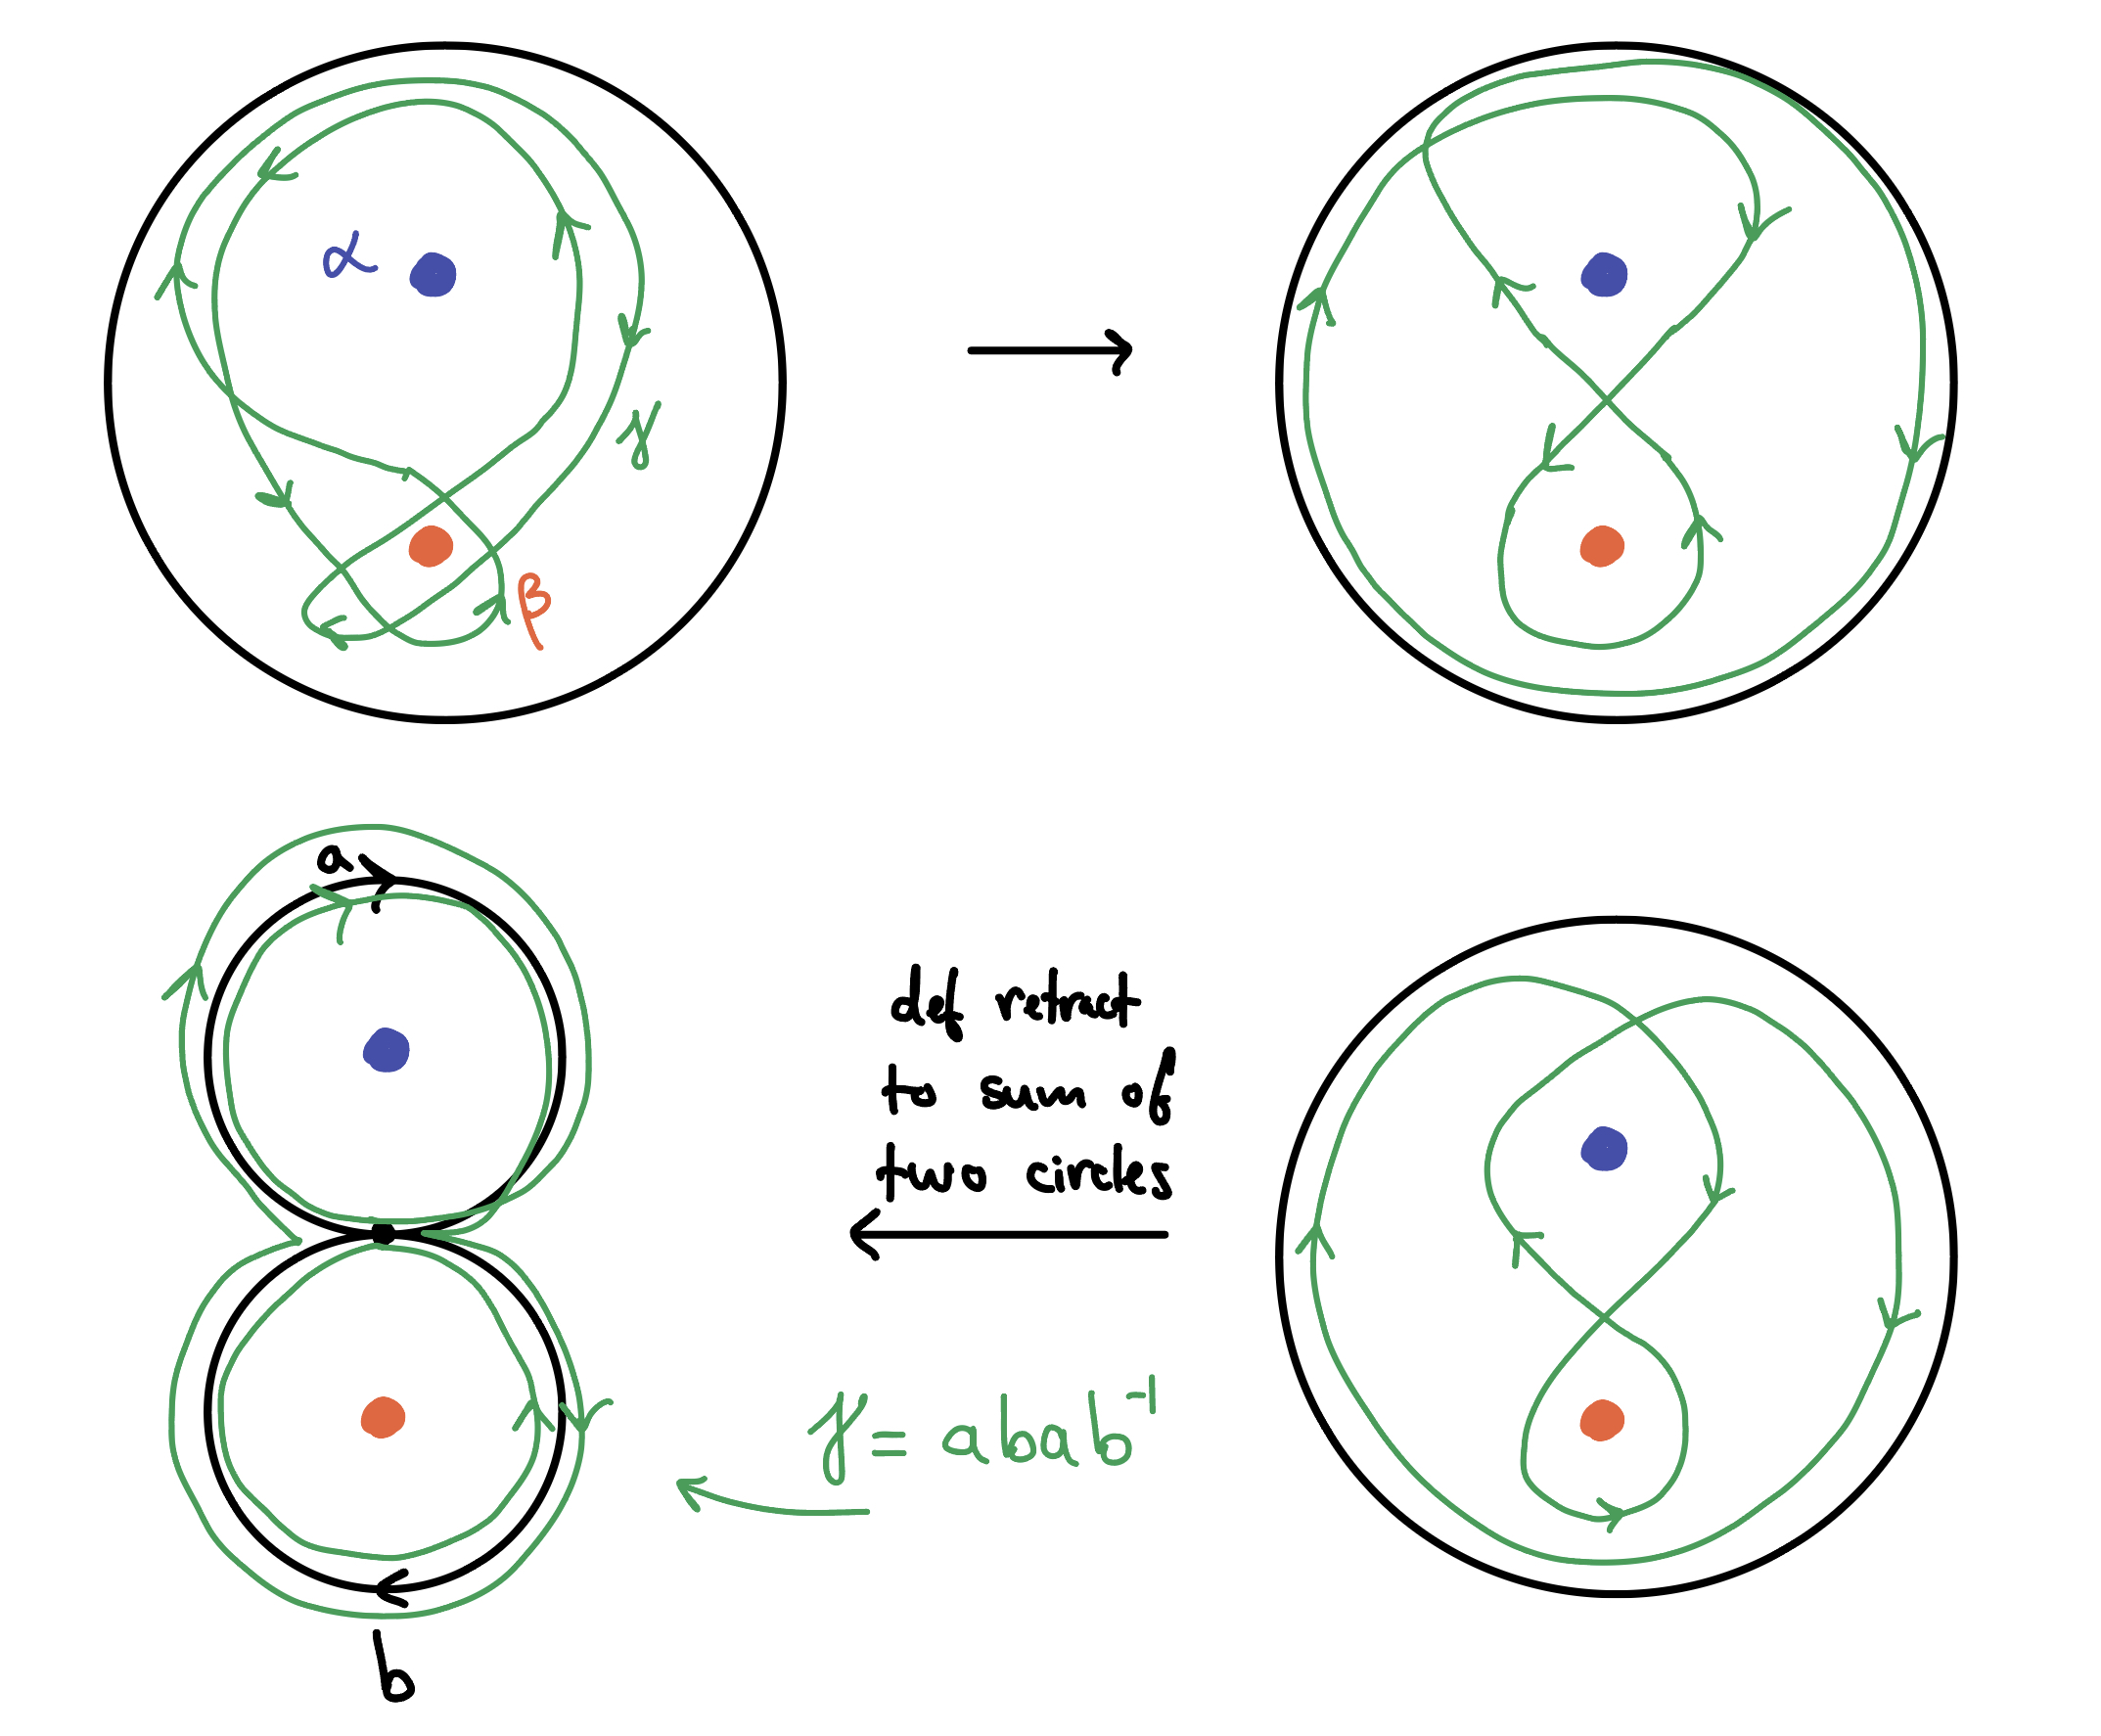
\includegraphics[width=14cm]{figures/hwk4-fig3.jpg}
      \captionof{figure}{Deformation retract of (5) onto $Y = D^2 - \{\alpha,\beta\}$}
      \label{fig:prob10.3}
    \end{center}
    Since we have a homotopy equivalence $D^2 \times I - (\alpha \cup \beta) \simeq S^1 \vee S^1$, we get an isomorphism $\pi_*(S^1\vee S^1) \cong \pi_*(D^2 \times I - (\alpha \cup \beta))$. Under this isomorphism, we can see that $\gamma$ is given by winding around $a$, $b$, again around $a$ and backwards around $b$, so $[\gamma] = abab^{-1} \in \pi_*(S^1\vee S^1)$. Because $\pi_*(S^1\vee S^1) \cong \bZ\ast \bZ$ and $abab^{-1}$ is a reduced word, $[\gamma]$ is not trivial in $\pi_*(S^1\vee S^1)$ and is hence not trivial in $D^1\times I - (\alpha \cup \beta)$.
  \end{prf}
  \prob[\textsc{Exercise 1.12}] The Klein bottle is usually pictured as a subspace of $\bR^3$ like the subspace $X \subseteq \bR^3$ shown in the first figure at the right. If one wanted a model that could actually function as a bottle, one would delete the open disk bounded by the circle of self-intersection of $X$, producing a subspace $Y \subseteq X$. Show that $\pi_1(X)\approx \bZ\ast \bZ$ and that $\pi_1(Y)$ has the presentation $\langle a,b,c ~\mid ~ aba^{-1}b^{-1}cb^\epsilon c^{-1} \rangle$ for $\epsilon = \pm 1$. (Changing the sign of $\epsilon$ gives an isomorphic group, as it happens.) Show also that $\pi_1(Y)$ is isomorphic to $\pi_1(\bR^3 - Z)$ for $Z$ the graph shown in the figure. The groups $\pi_1(X)$ and $\pi_1(Y)$ are not isomorphic, but this is not easy to prove; see the discussion in Example 1B.13.
  \begin{prf}
    We first demonstrate that the Klein bottle has fundamental group isomorphic $\bZ\ast \bZ$. We do this by showing $X \simeq S^2 \vee S^1 \vee S^1$ via a series of intermediate homotopy equivalences. This is justified in Figure (\ref{fig:prob12.1}).
    \begin{center}
      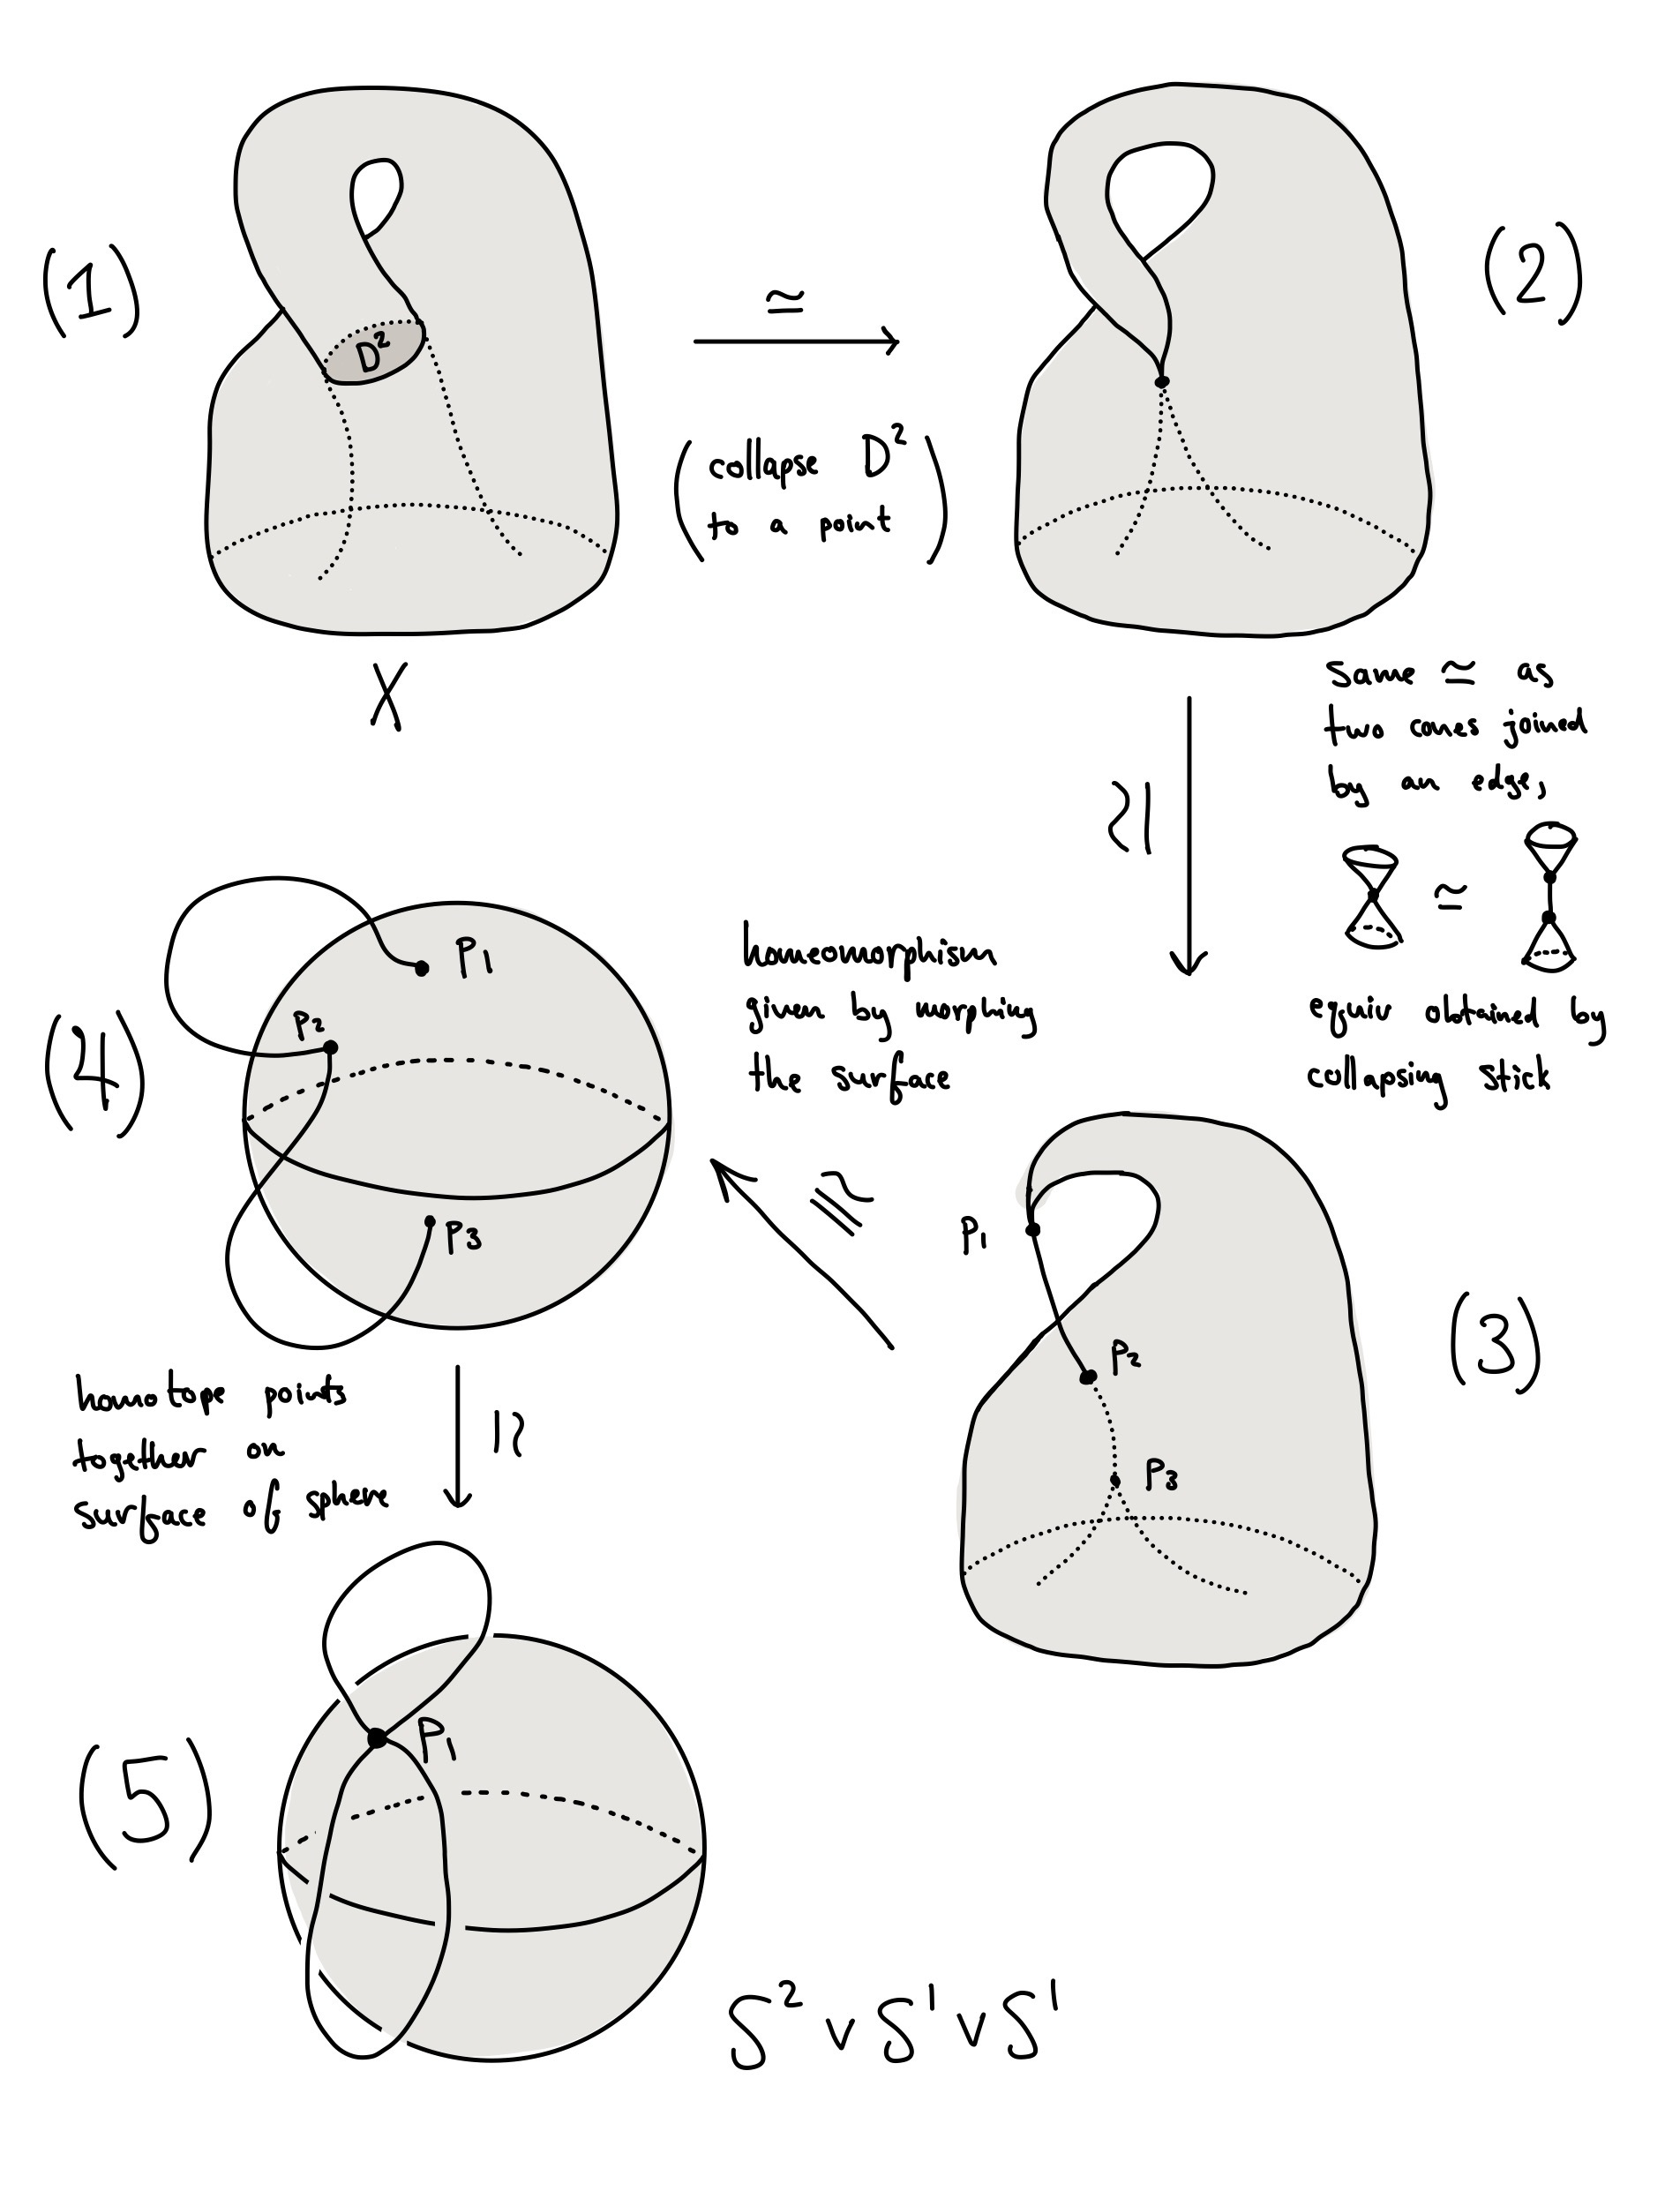
\includegraphics[width=14cm]{figures/hwk4-fig6.jpg}
      \captionof{figure}{Homotopy equivalence of the Klein bottle to $S^2 \vee S^1 \vee S^1$}
      \label{fig:prob12.1}
    \end{center}
    Hence $\pi(X) \cong \pi_1(S^2 \vee S^1 \vee S^1) \cong \bZ \ast \bZ$.

    Now let $Y$ be $X$ obtained by deleting the open disk of self intersection on the surface of $X$. To calculate the fundamental group of $Y$, we modify the usual cell complex used for the Klein bottle to include a third 1-cell. 
    \begin{center}
      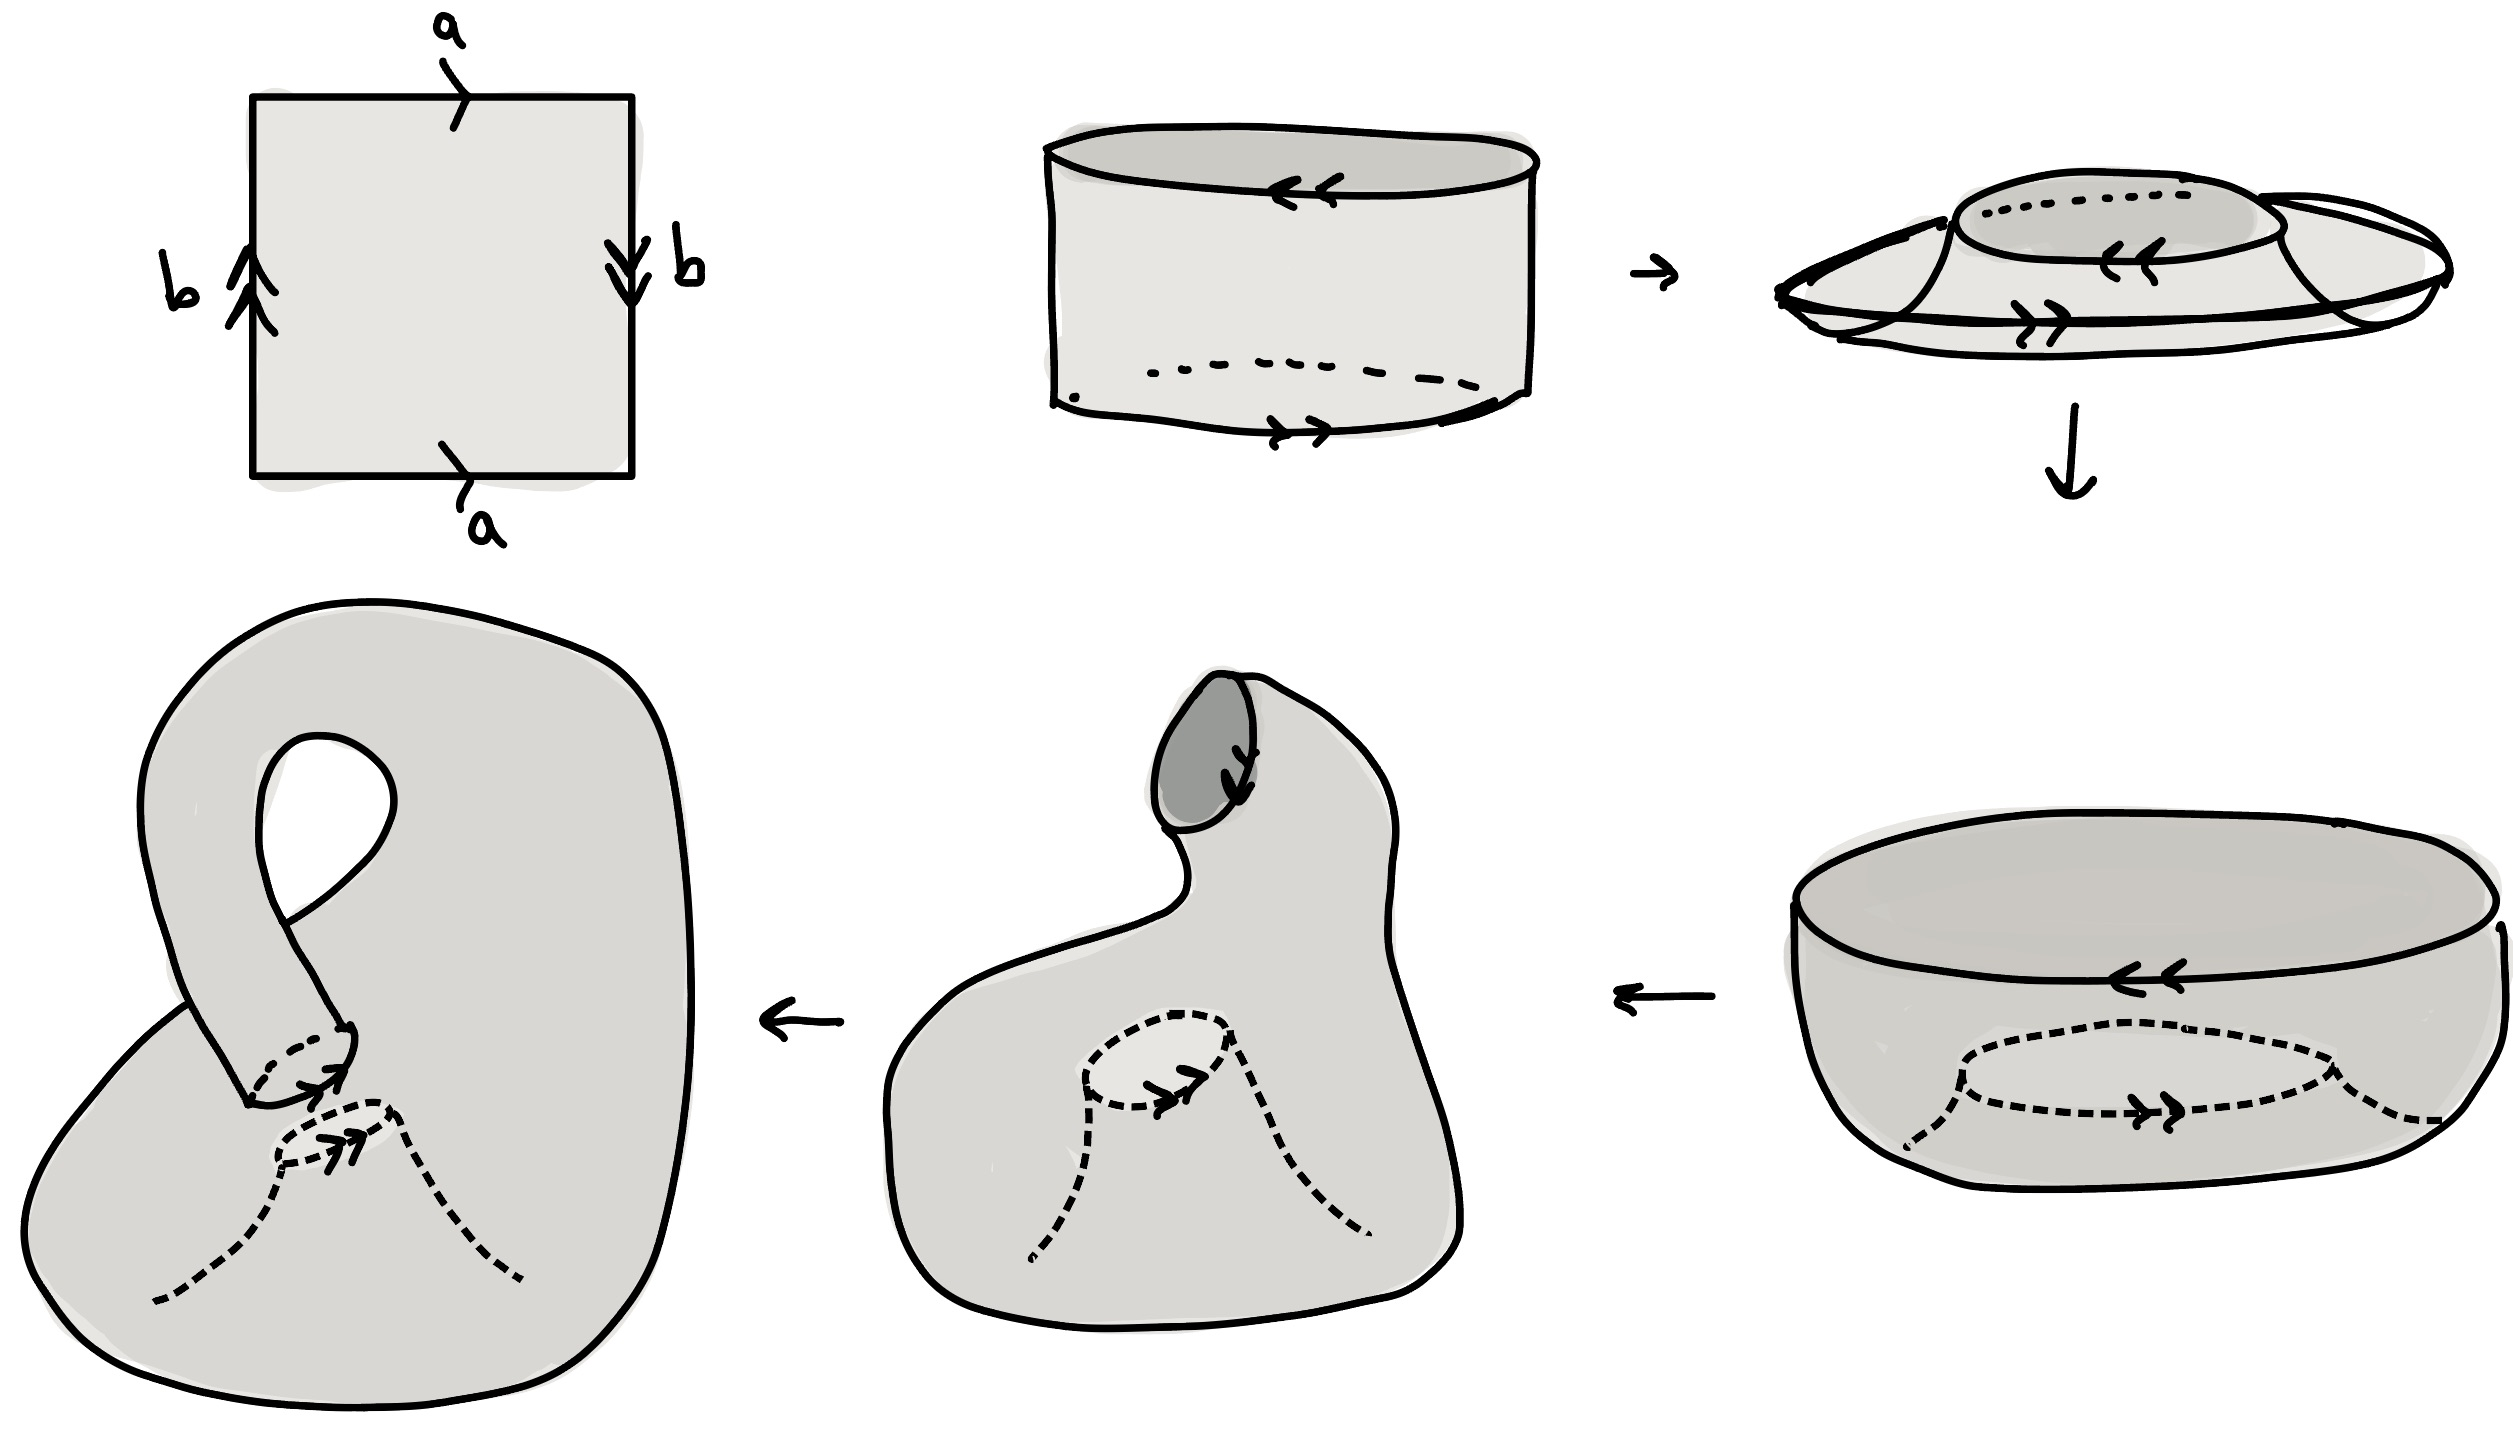
\includegraphics[width=14cm]{figures/hwk4-fig7.png}
      \captionof{figure}{The typical identification used to construct the Klein bottle}
      \label{fig:prob1.2.12}
    \end{center}
    It is clear that we need to add a $1$-cell, as some loops which were previously homotopic to the trivial loop prior to the deletion of the self-intersection disk are no longer trivial. However, I'm not entirely sure how the identification map $S^1\to X^1$ should be defined. Proposition 1.26 tells us that it ought to map the boundary to $aba^{-1}b^{-1}cb^{\epsilon}c^{-1}$, as this is the relation in the problem statement, but I'm having a difficult time seeing what space this boundary map produces.
    \begin{center}
      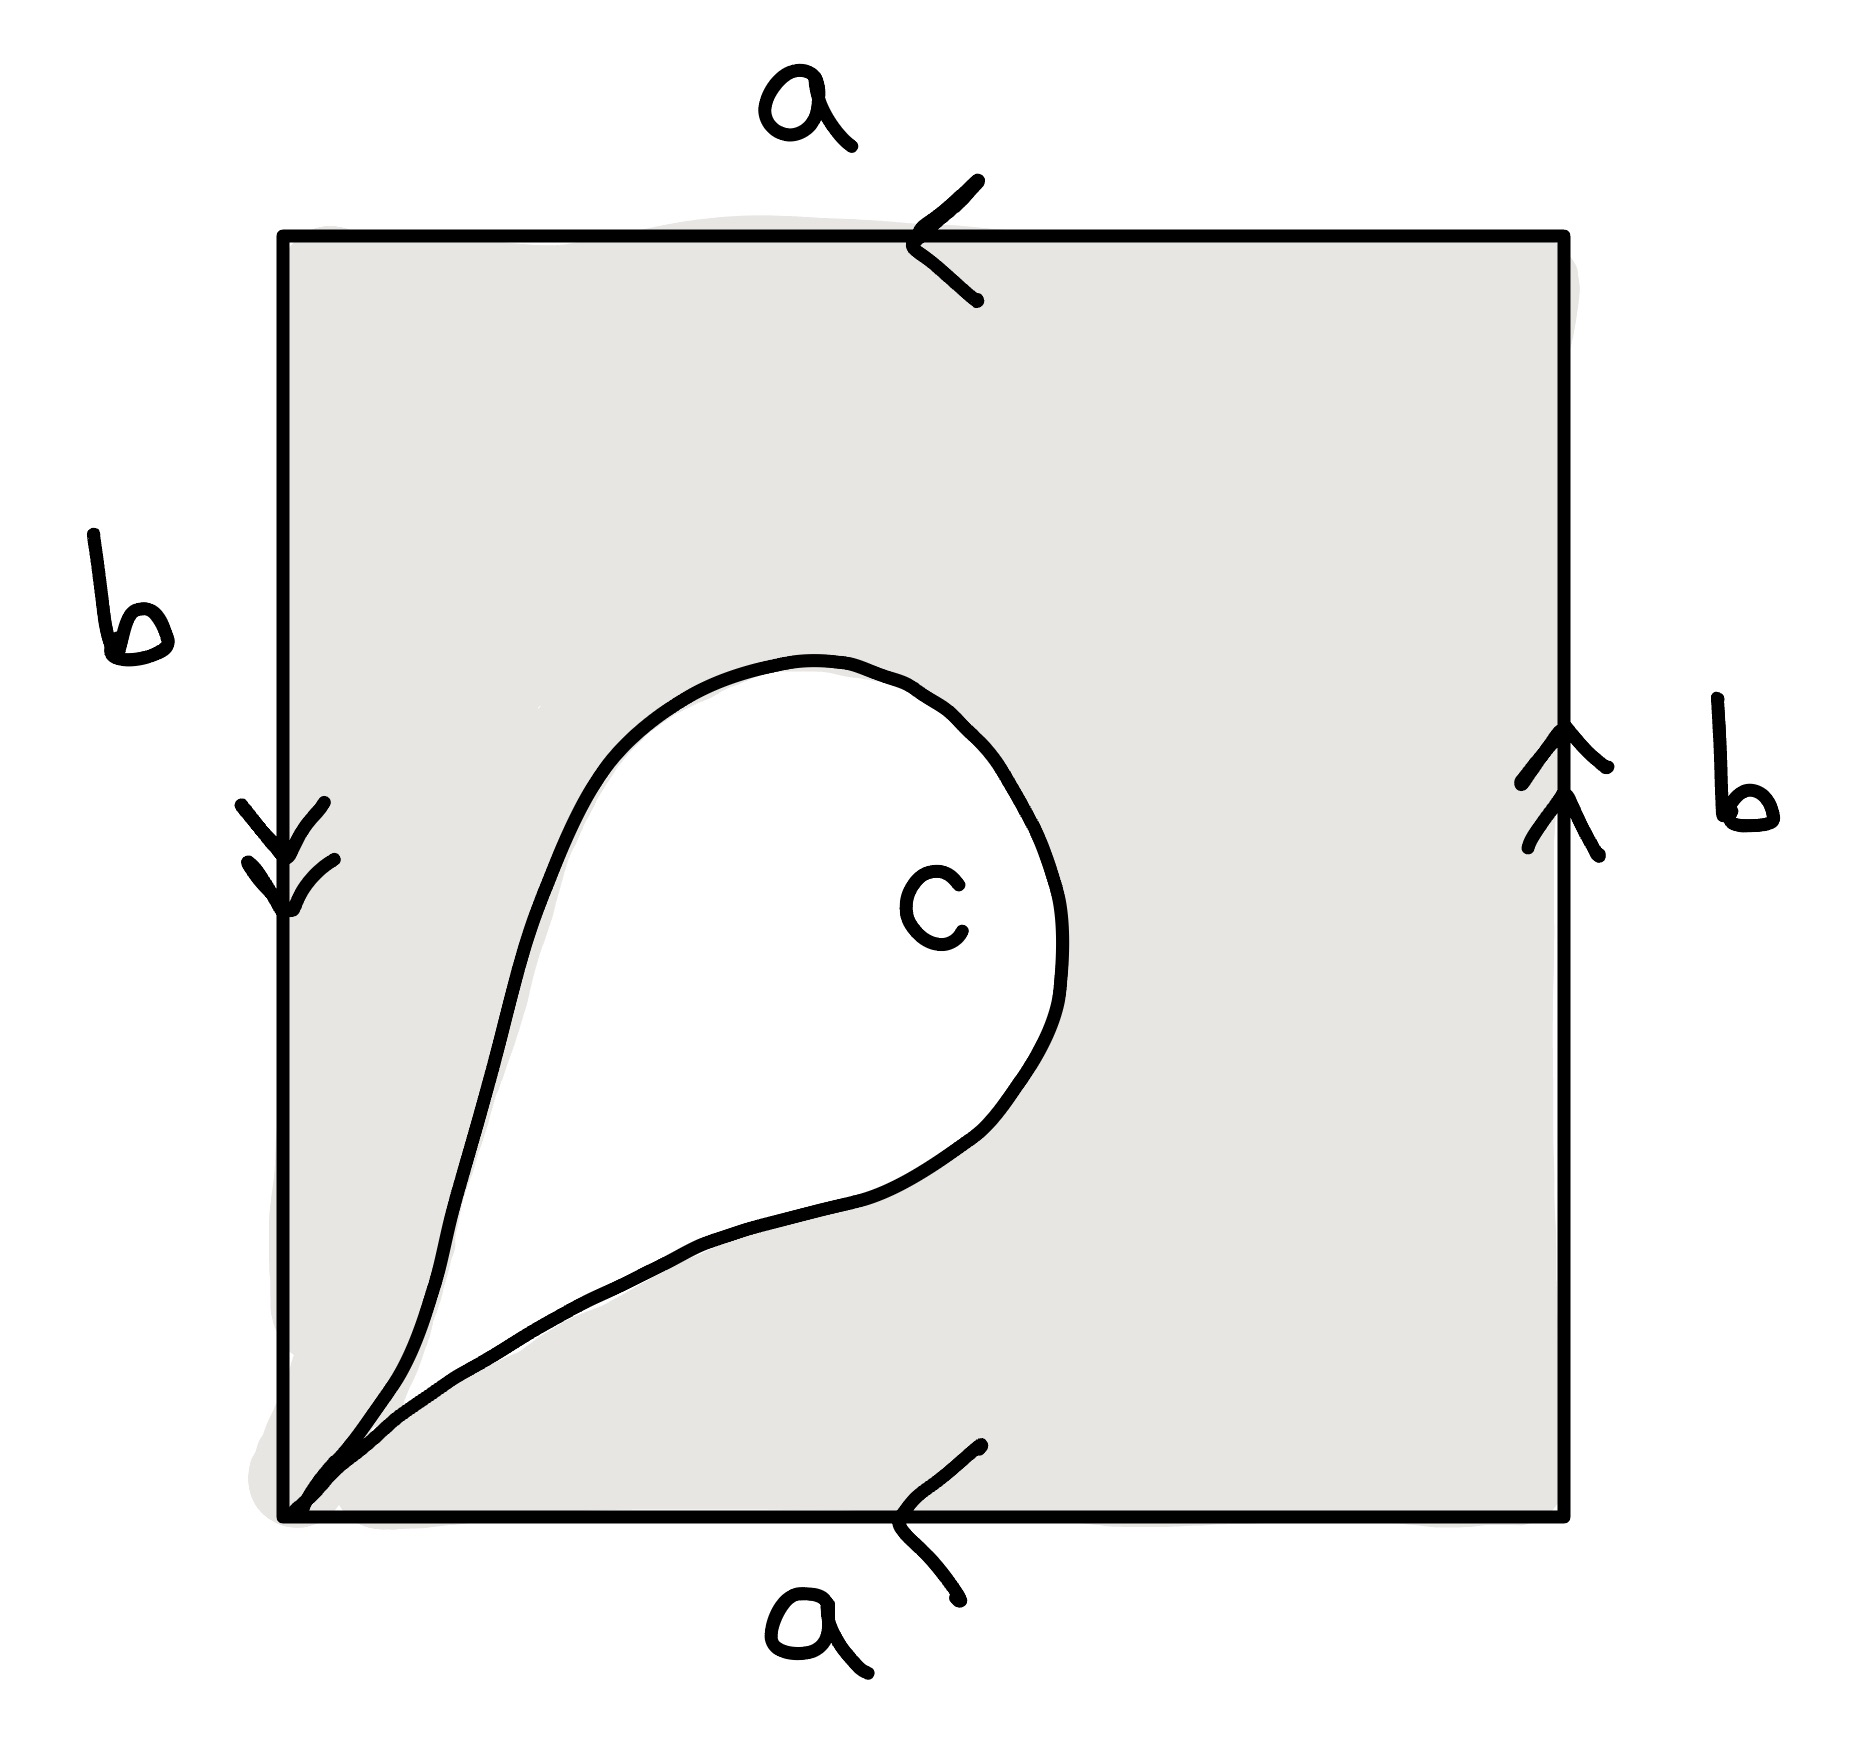
\includegraphics[width=8cm]{figures/hwk4-fig8.png}
      \captionof{figure}{The typical identification of the Klein bottle used with an extra $1$-cell.}
      \label{fig:prob1.2.12.1}
    \end{center}
  \end{prf}

  \newpage
  \prob[\textsc{Exercise 1.14}] Consider the quotient space of a cube $I^3$ obtained by identifying each square face with the opposite square face via the right-handed screw motion consisting of a translation by one unit in the direction perpendicular to the face combined with a one-quarter twist of the face about its center point. Show this quotient space $X$ is a cell complex with two $0$-cells, four $1$-cells, three $2$-cells, and one $3$-cells. Using this structure, show that $\pi_1(X)$ is the quaternion group $\{\pm 1, \pm i, \pm j,\pm k\}$, of order eight.
  \begin{prf}
    Realizing the $1$-skeleton of $X$ is not terribly difficult. After making the face identifications by right-handed screw motions, we see that each of the 12 edges gets identified to 2 other edges, leaving a total of 4 distinct edges. This gives us the one skeleton, pictured in figure (\ref{fig:prob14.1}). 
    \begin{center}
      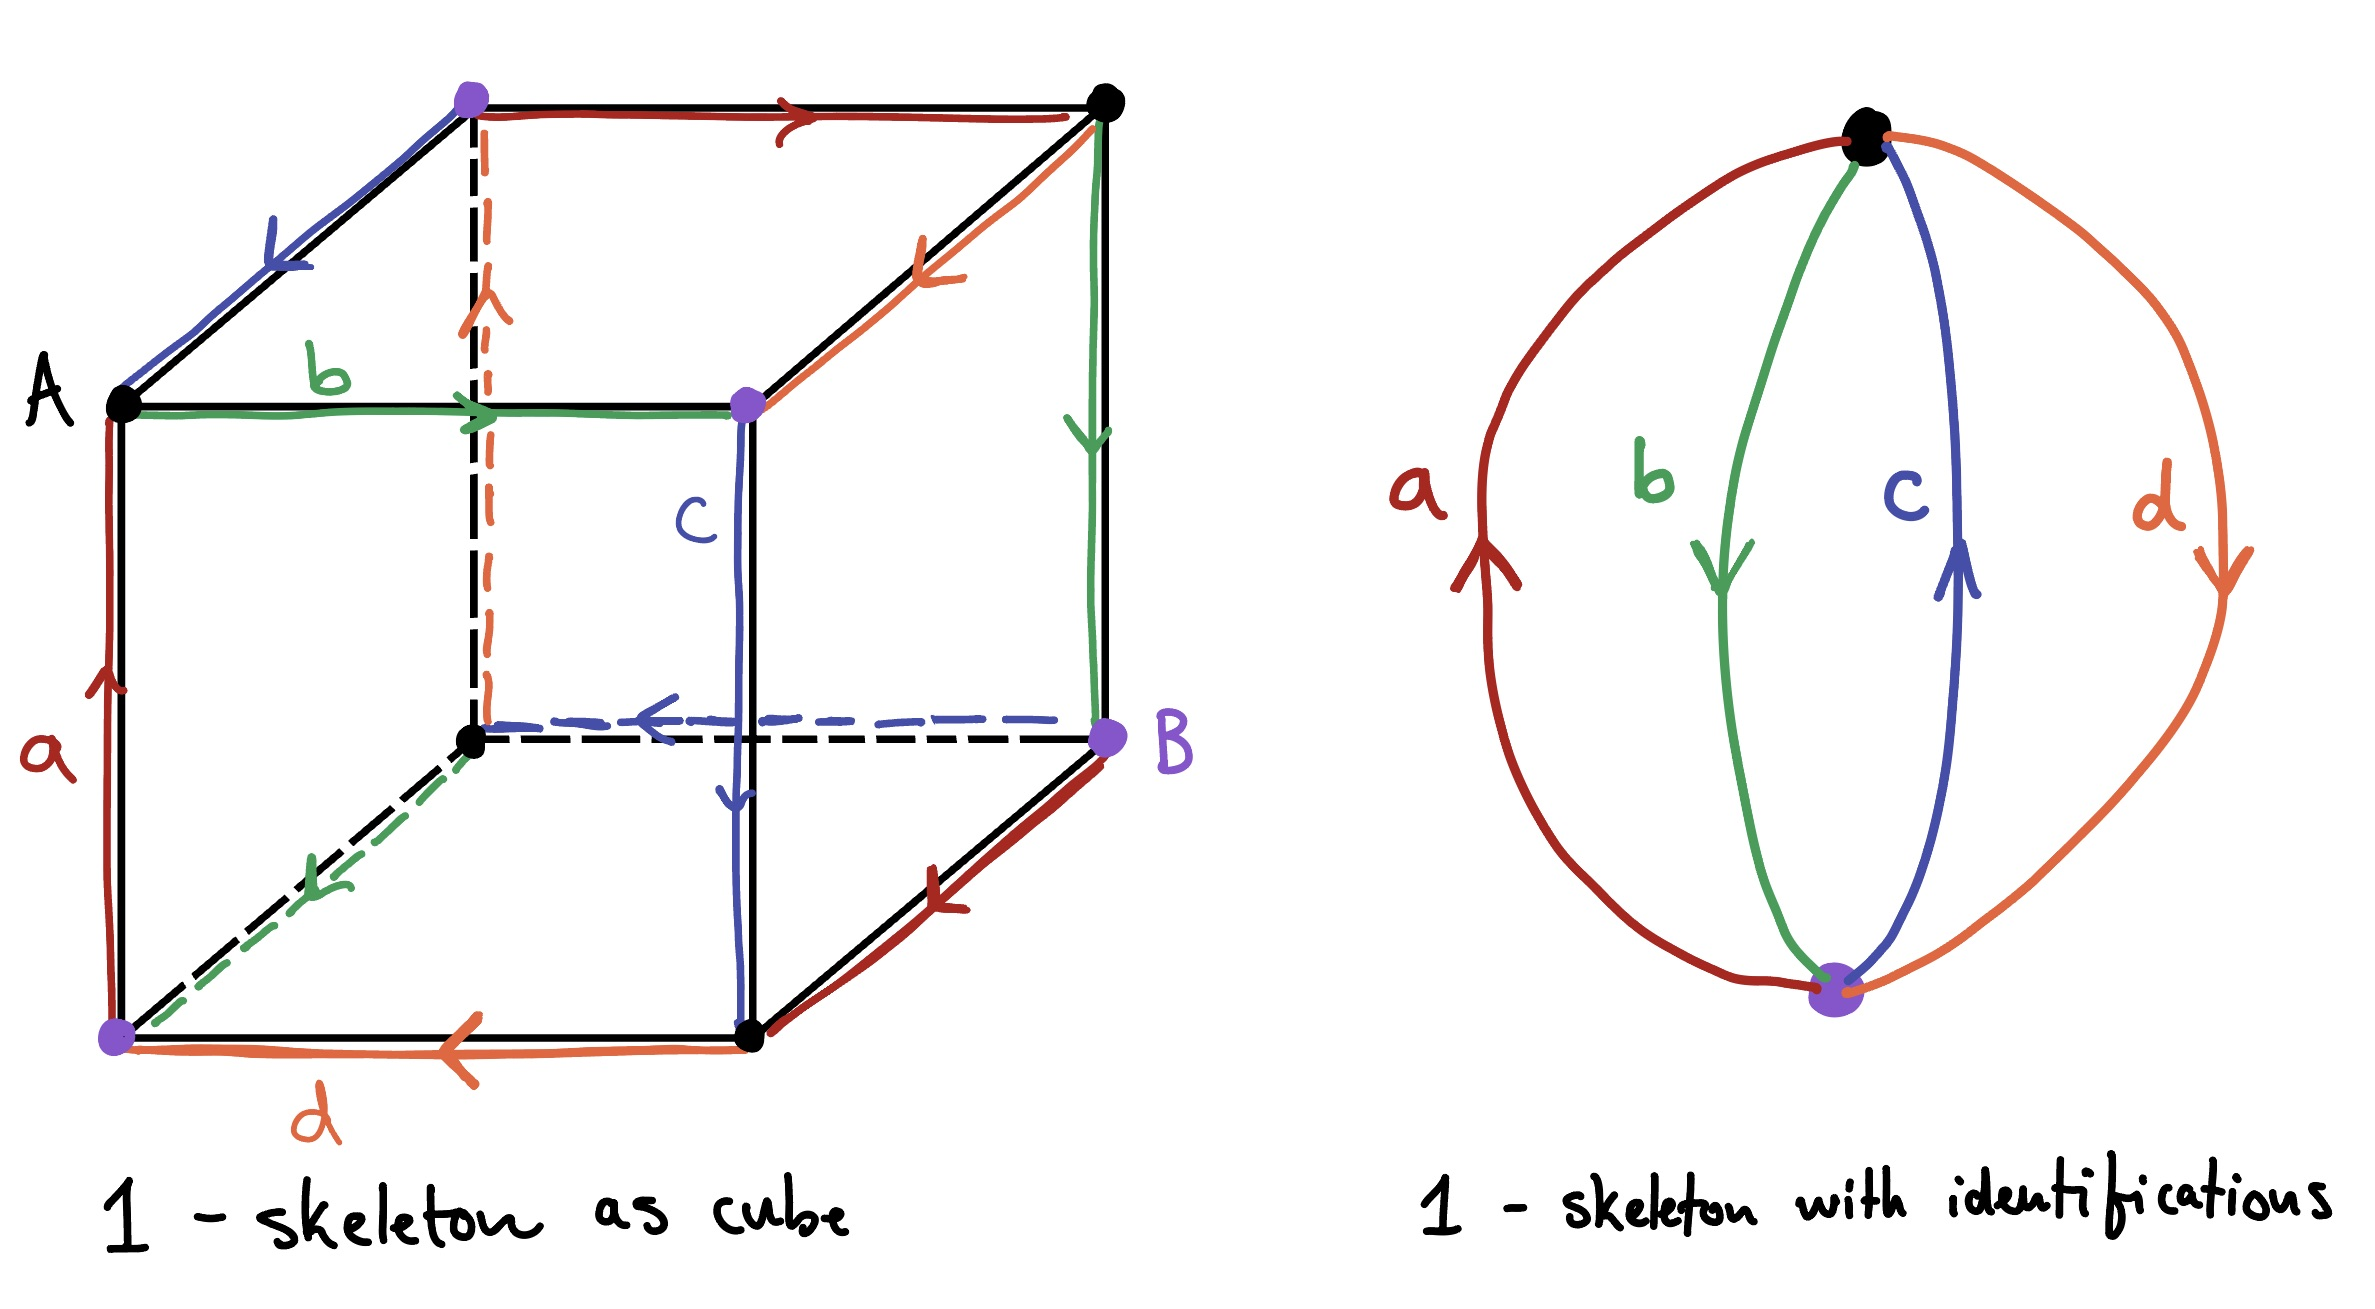
\includegraphics[width=14cm]{figures/hwk4-fig4.jpg}
      \captionof{figure}{The one skeleton $X^1$}
      \label{fig:prob14.1}
    \end{center}
    We can easily calculate $\pi_1(X^1)$ by realizing it is the deformation retract of disk with three points removed, which also deformation retracts to the wedge of three circles.
    \begin{center}
      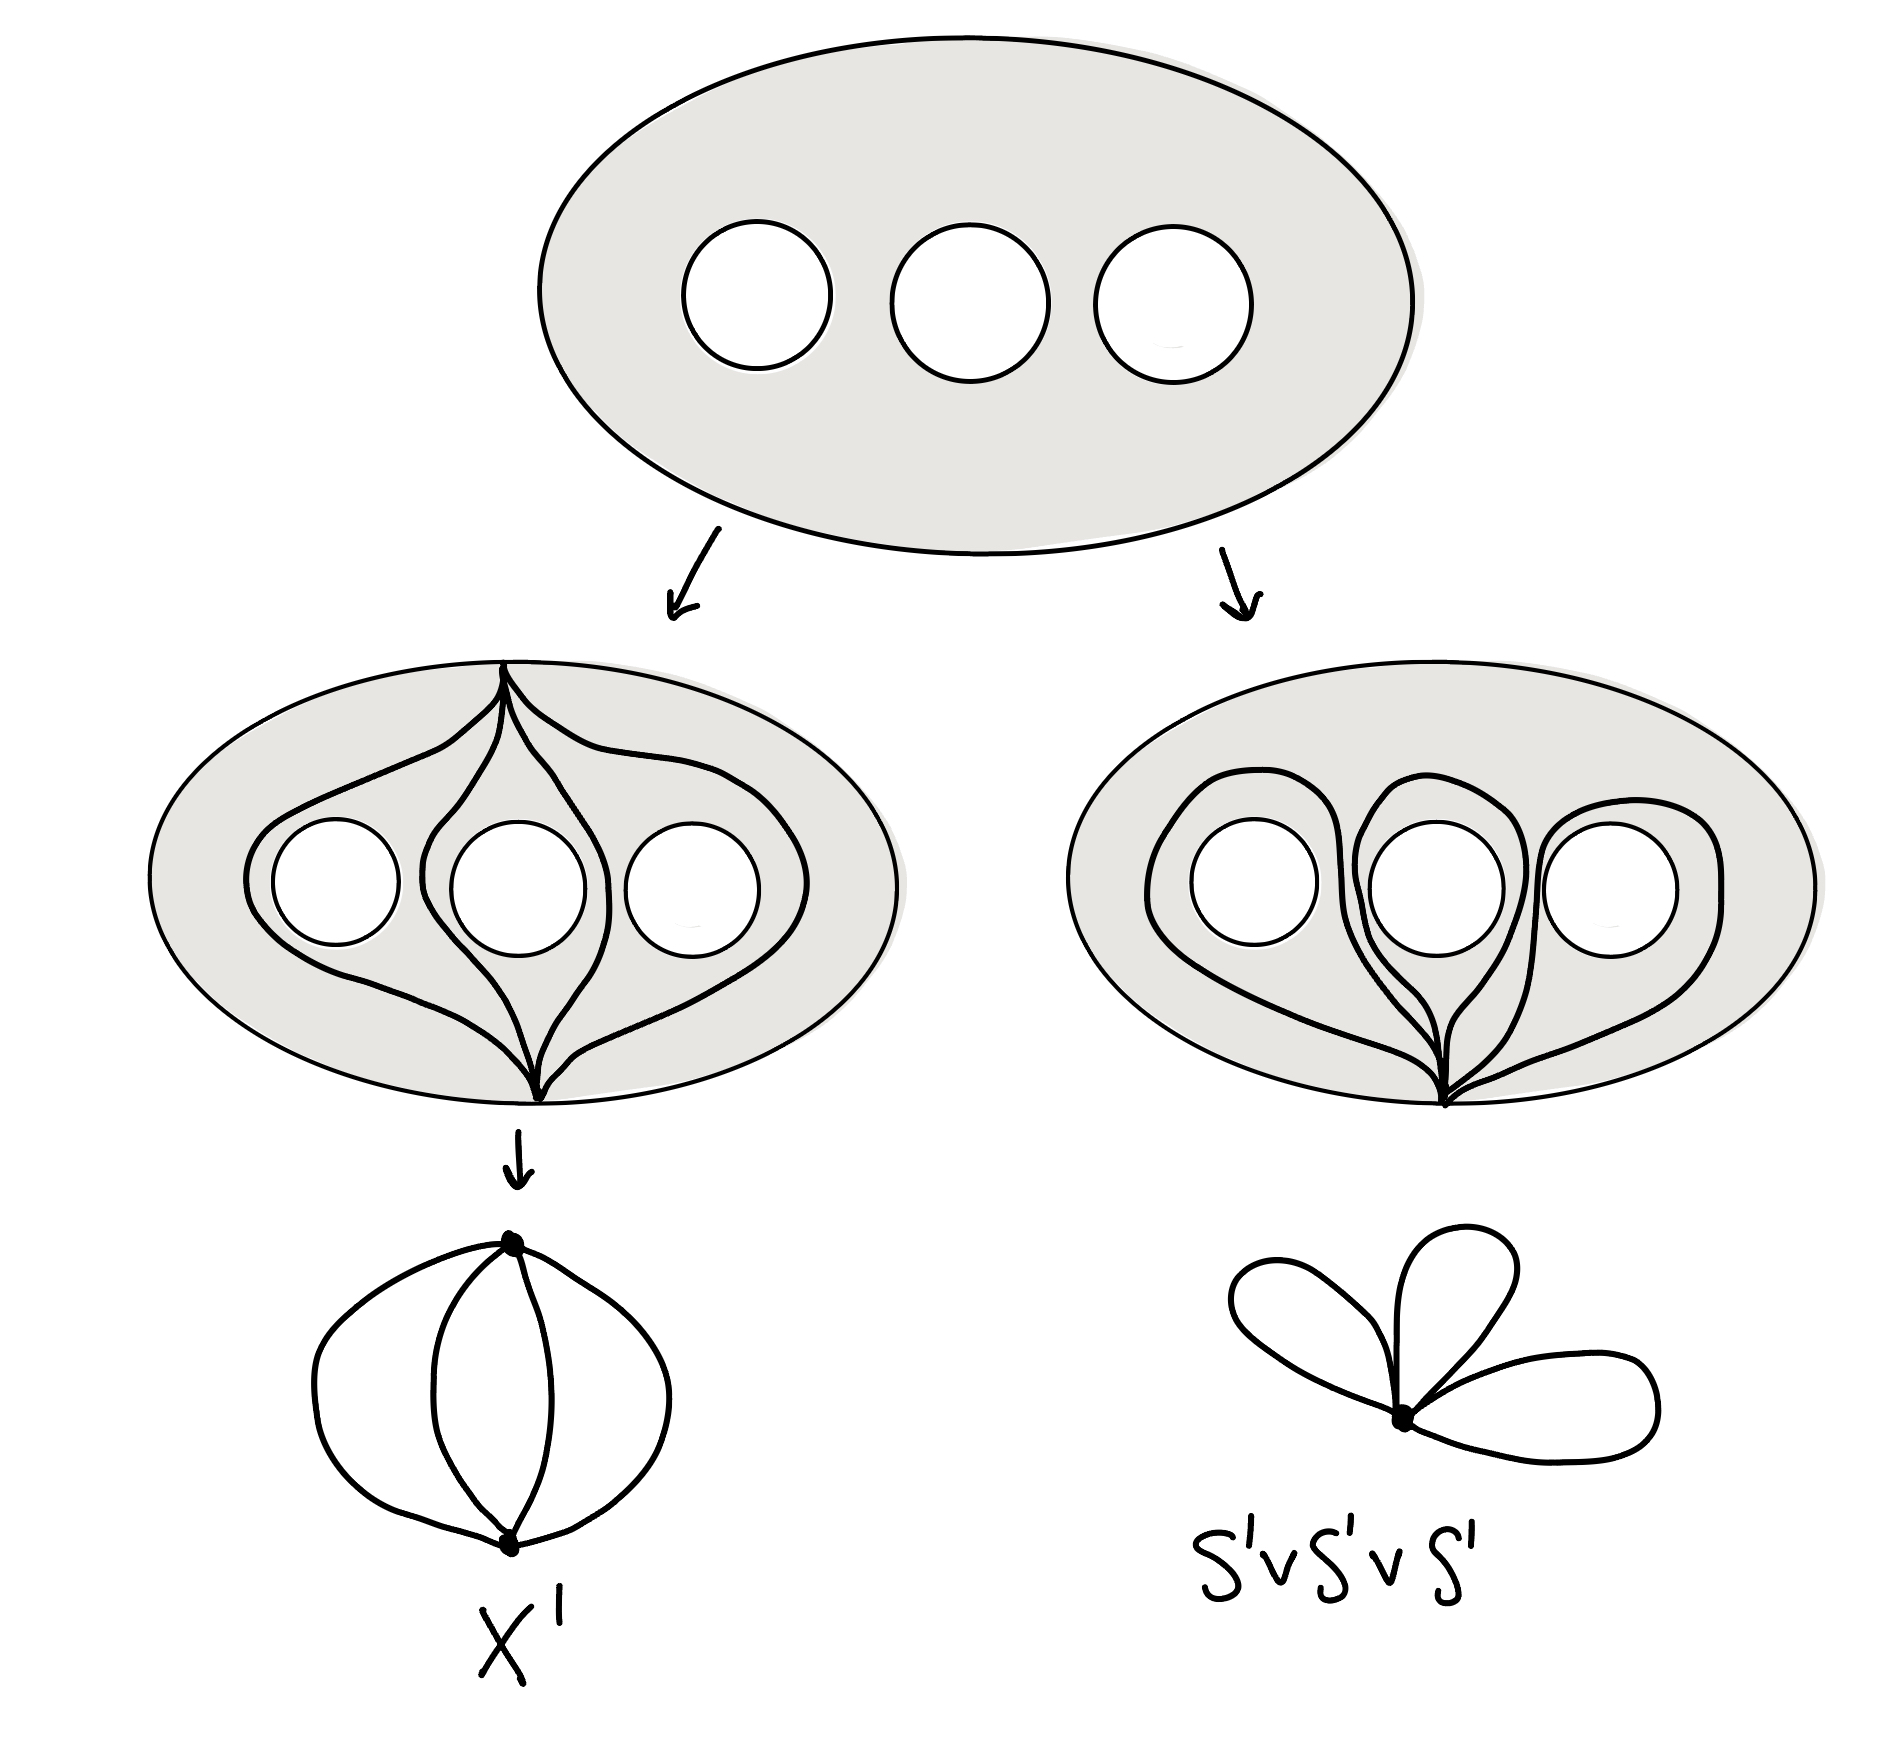
\includegraphics[width=14cm]{figures/hwk4-fig5.jpg}
      \captionof{figure}{The one skeleton $X^1$}
      \label{fig:prob14.2}
    \end{center}
    The transitivity of homotopy equivalence implies that $\pi_1(X^1) \cong \pi_1(S^1\vee S^1\vee S^1) \cong \bZ\ast \bZ\ast \bZ$. Choosing the purple point in Figure (\ref{fig:prob14.1}) as out basepoint, the generators of $\pi_1(X^1)$ are $x = [ab], y = [cb]$ and $z = [cd]$.

    We now attach the $2$-cells to $X^1$. These will correspond to the faces of the cube, of which there are only three post-identification. Van Kampen's theorem tells us that each loop around a face in $X$ can be regarded either as a loop in $X^1$ or as a loop contained entirely in the $2$-cell in question, so we must identify all such loops. Consider the front face in Figure (\ref{fig:prob14.1}). It has boundary loop $[abcd]$, which must be equal to $1$ in the fundamental group of the $2$-cell. Hence, in $\pi_1(X^2)$,
    \begin{align*}
      1 = [abcd] = [ab][cd] = xz.
    \end{align*}
    The boundary loops for the top and right faces of the cube are given by $b^{-1}c^{-1}ad$ and $ca^{-1}b^{-1}d$ respectively. Setting these to $1$ give
    \begin{align*}
      1 = [b^{-1}c^{-1}ad] = [cb]^{-1}[ab][b^{-1}c^{-1}][cd] = y^{-1}xy^{-1}z \implies yz^{-1} = xy^{-1}
    \end{align*}
    and
    \begin{align*}
      1 = [ac^{-1}d^{-1}b] = [ab][cb]^{-1}[ad]^{-1}[ab] = xy^{-1}z^{-1}x
    \end{align*}
    so $yz^{-1} = xy^{-1}$ and $xy^{-1}z^{-1}x = 1$. At this point it is convenient to change our generators, instead of $x,y$ and $z$ we will use $i = [ab]$, $j = [ac^{-1}]$ and $k = [ad]$. These also generate $\pi_1(X^2)$ since
    $x = i$, $y = j^{-1}i$, $z = j^{-1}k$. The relations we found above become
    \begin{align*}
      xz = 1 &\rightsquigarrow ij^{-1}k = [ab][ca^{-1}][ad] = [ab][cd] = xz = 1 \implies j = ki\\
      yz^{-1} = xy^{-1} &\rightsquigarrow (j^{-1}i)(k^{-1}j) = (i)(i^{-1}j) \implies i = jk \\
      xy^{-1}z^{-1}x = 1 &\rightsquigarrow  (i)(i^{-1}j)(j^{-1}k)(j^{-1}i^{-1}) = 1 \implies k = ij.
    \end{align*}
    Hence, by Proposition 1.26 in Hatcher,
    \begin{align*}
      \pi_1(X^2) = \frac{\pi_1(X^1)}{\langle k^{-1}ji^{-1}, i^{-1}kj^{-1},k^{-1}j^{-1}i \rangle} = \langle i,j,k ~\mid~ i=jk, k = ij \rangle.
    \end{align*}
    From here we can see that we have a presentation of the quanternion group, since
    \begin{align*}
      i^2 = i(jk) = ijk \hspace{1em}&,\hspace{1em} k^2 = (ij)k = ijk \\
      j = ki = k(jk) = kjk \hspace{1em}&,\hspace{1em} j^2 = (jk)jk = ijk.
    \end{align*}
    Thus $\pi_1(X^2) = \langle i,j,k ~\mid~ i^2 = j^2 = k^2 = ijk \rangle$. Attaching the three cell to $X^2$to obtain $X$ does not change the fundamental group, so $\pi_1(X) \cong \pi_1(X^2)$ is the quanternion group.
  \end{prf}
  \prob[\textsc{Exercise 1.21}] Show that the join $X*Y$ of two nonempty space $X$ and $Y$ is simply-connected if $X$ is path-connected.
\begin{proof}
    Let $(x,y,t),(u,v,s) \in X * Y$. We regard $X * Y$ as the space $X \times Y \times I / \sim$ where $(x,y_1,0) \sim (x,y_2,0)$ and $(x_1,y,1) \sim (x_2,y,1)$.
    
    We first show that $X * Y$ is path connected.  There exists a path from $(x,y,t)$ to $(x,y,0)$, call it $\gamma_1$. Because $X$ is path connected, there exists a path from $(x,y,0)$ to $(u,y,0)$ which is identified with $(u,v,0)$ in $X * Y$. We call the path from $(x,y,0)$ to $(u,v,0)$ $\gamma_2$. Finally, call the path from $(u,v,0)$ to $(u,v,s)$ $\gamma_3$. The path $\gamma_3 \gamma_2 \gamma_1$ starts at $(x,y,t)$ and ends at $(u,v,s)$. Therefore, there is path connecting any two points in $X*Y$, so $X*Y$ is path connected.  
    
    In order to apply Van Kampen's theorem, we must make a choice of open sets with which to express $X * Y$. These ought to be open sets whose intersection has a familiar fundamental group. Let $A = X \times Y \times [0,1) / \sim$ and $B = X \times Y \times (0,1] / \sim$. These sets are open, and their intersection is precisely $X \times Y \times (0,1)$ \emph{without} the equivalence relation. Since we can continuously retract the copies of $I$ extending from $X$ down onto $X$, we can deformation retract $A$ onto $X$. Similarly, we can deformation retract $B$ onto $Y$. This is similar to the process in problem 0.6(a) in Hatcher. Finally, by retracting either end of the intervals onto the point \{1/2\}, we can deformation retract $A \cap B$ to $X \times Y \times \{\frac{1}{2}\}$, which is homeomorphic to $X \times Y$. 
    
    This means $\pi_1(A \cap B) \approx \pi_1(X) \times \pi_1(Y)$, $\pi_1(A) \approx \pi_1(X)$, and $\pi_1(B) \approx \pi_1(Y)$. Van Kampen tells us that 
    \begin{equation*}
        \pi_1(X*Y) \approx \pi_1(A) * \pi_1(B) / N 
    \end{equation*}
    where $N$ is generated by elements of the form $\iota_A(\omega)\iota_B(\omega)^{-1}$ where $\iota_A: \pi_1(A \cap B) \hookrightarrow \pi_1(A)$ and 
    
    \noindent
    $\iota_B: \pi_1(A \cap B) \hookrightarrow \pi_1(B)$ are the homomorphisms induced by the inclusions. However, as we concluded above, $\pi_1(A \cap B) \approx \pi_1(X) \times \pi_1(Y)$. This means that $\iota_A$ and $\iota_B$ are actually surjective projections, and therefore the elements of the form $\iota_A(\omega)\iota_B(\omega)^{-1}$ are equivalently $ab^-1$, $a \in \pi_1(A)$ and $b \in \pi_1(B)$ . By modding out by $N$ we are thus actually identifying \emph{all} points. Thus, 
    
    \begin{equation*}
        \pi_1(X * Y) \approx \pi_1(A) * \pi_1(B) / N = 1
    \end{equation*}
\end{proof}

\newpage
\end{homework}
\tchap{Extra Problem}
\begin{homework}[e]
  \prob The Dehn presentation of a $\pi_1(\bR^3-L)$, for $L$ a link, is different
    from the more popular
    Wirtinger presentation (see Hatcher's \S1.2\#22).
    I personally think it is easier to understand.

    Write $p$ for the projection $\bR^3\to\bR^2$. Suppose the projection
    of $L$ has the usual form for a link diagram.  In particular, $L$ lies
    in the plane $\bR^2$, except near crossings, where one strand is
    slightly higher than the other.
    Then $p(L)$ divides $\bR^2$
    into components.  
    The Dehn presentation has one generator for each bounded component.
%    (We take the identity element as the ``generator'' associated to the
%    unbounded region.)
    There is one relation for each crossing.  Suppose the regions involved
    at that crossing are $A,B,C,D$ as in the picture.  The relation is
    $AB^{-1}CD^{-1}=1$.
    \begin{center}
        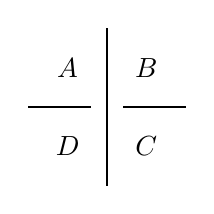
\begin{tikzpicture}
            \draw(-1,0)--(-.2,0);
            \draw(1,0)--(.2,0);
            \draw(0,1)--(0,-1);
            \draw(-.5,.5) node {$A$};
            \draw(.5,.5) node {$B$};
            \draw(.5,-.5) node {$C$};
            \draw(-.5,-.5) node {$D$};
        \end{tikzpicture}
    \end{center}
    (One or more of the four quadrants involved at a crossing might be
    the unbounded
    region. For each such quadrant, use the same relation, but with
    the identity element $1$ as the ``generator'' corresponding to that region.)
    Prove that this presentation gives $\pi_1(\bR^3-L)$.

    A simple example for you to
    work out to understand things takes $L$ to be the trefoil knot. You'll
    have 4 generators and 3 relations, each relation having length~$3$.
    You should be drawing pictures
    like mad throughout this problem.

    Here is the meaning of the generators.  We take the basepoint to
    be far above the plane. 
    Each generator goes down from the basepoint,
    down through a point of the corresponding
    region, and then comes back up through the unbounded region and returns
    to the basepoint.
    %(This is why the ``generator'' associated to the outside region is the identity.)

    \medskip
    Here is  an approach to proving that the
    presentation is legit.  We start by building a $2$-complex~$X$ containing~$L$.
    Its $1$-skeleton is the union of $L$ and one vertical segment for each 
    crossing, joining the upper strand to the lower strand at that crossing.
    For a given bounded 
    region $R$, consider the portion of $L$ that projects to $\partial R$. 
    It is a union of segments.  The endpoints of these segments map $2$-to-$1$
    to the corners of~$R$. The union
    of these arcs along $L$, together with the vertical segments joining pairs
    of endpoints, form a circle.  Attach a $2$-cell along this loop.  You
    can do this in $\bR^3$, with the disk lying in $\bR^2$ except near the corners of~$R$, where it twists a bit.  

    First show  $\pi_1(\bR^3-X)=1$.  
    Then work out $\pi_1(\bR^3-X^1)$, where $X^1$ is
    the $1$-skeleton.  One way to do this is to  adjoin to $\bR^3-X$ an open
    neighborhood of each of my supposed  generators for $\pi_1$. 
    You should find that $\pi_1(\bR^3-X^1)$ is free on the set of bounded regions. 
    Then you work out $\pi_1(\bR^3-L)$ by adjoining to $\bR^3-X^1$ a small open
    neighborhood of each of the vertical segments in $X^1$. 
    
    This approach is ``dual'' to the usual approach of ``$1$-cells are generators,
    $2$-cells are relations''.  To use the usual approach, one can find a sort
    of ``dual'' complex to~$X$ in $\bR^3$, to which $\bR^3-L$ deformation-retracts.
    But 
    I have an easier time seeing the relation by the approach above, because they are
    represented by very small loops around the vertical segments.
\begin{prf}
  As suggested, we first show that $\pi_1(\bR^3 - X) = 1$, where $X$ is the $2$-complex constructed in the problem statement. We first deformation retract the vertical segments attached to the crossings to points. This doesn't affect the fundamental group of $X$, and it results in the identification of the crossing points. We then get a projected link with its bounded regions all filled, which is homeomorphic to a disk, and hence homotopy equivalence to a point. This implies that $\pi_1(\bR^3 - X) \cong \pi_1(\bR^3 - \text{pt}) = 1$, since $\bR^3 - \text{pt}$ deformation retracts to $S^2$.

  We now argue that we ought to have a generator for each region in $X^1$ using Van Kampen. Fix a bounded region $R$ (homeomorphic to a disk) and consider taking a loop $\gamma$ passing under and over $R$ as described in the problem statement. Let $C$ be a slight enlargement of $\gamma$, a cylinder surrounding $\gamma$, and set $U = C \cup R$. This space deformation retracts to $\gamma$, hence $\pi_1(U) = \bZ$. Now set $V = \bR^3 - X$. This space is simply connected by what we've already shown. Likewise, the space $U\cap V = C - R$ deformation retracts to a disk, as it is a cylinder with a cross section deleted, and therefore also has trivial fundamental group. By Van Kampen, we therefore have that $\pi_1(U \cup V) \cong \bZ$, indicating that we need to add a generator for each bounded region in $X - L$.
    \begin{center}
      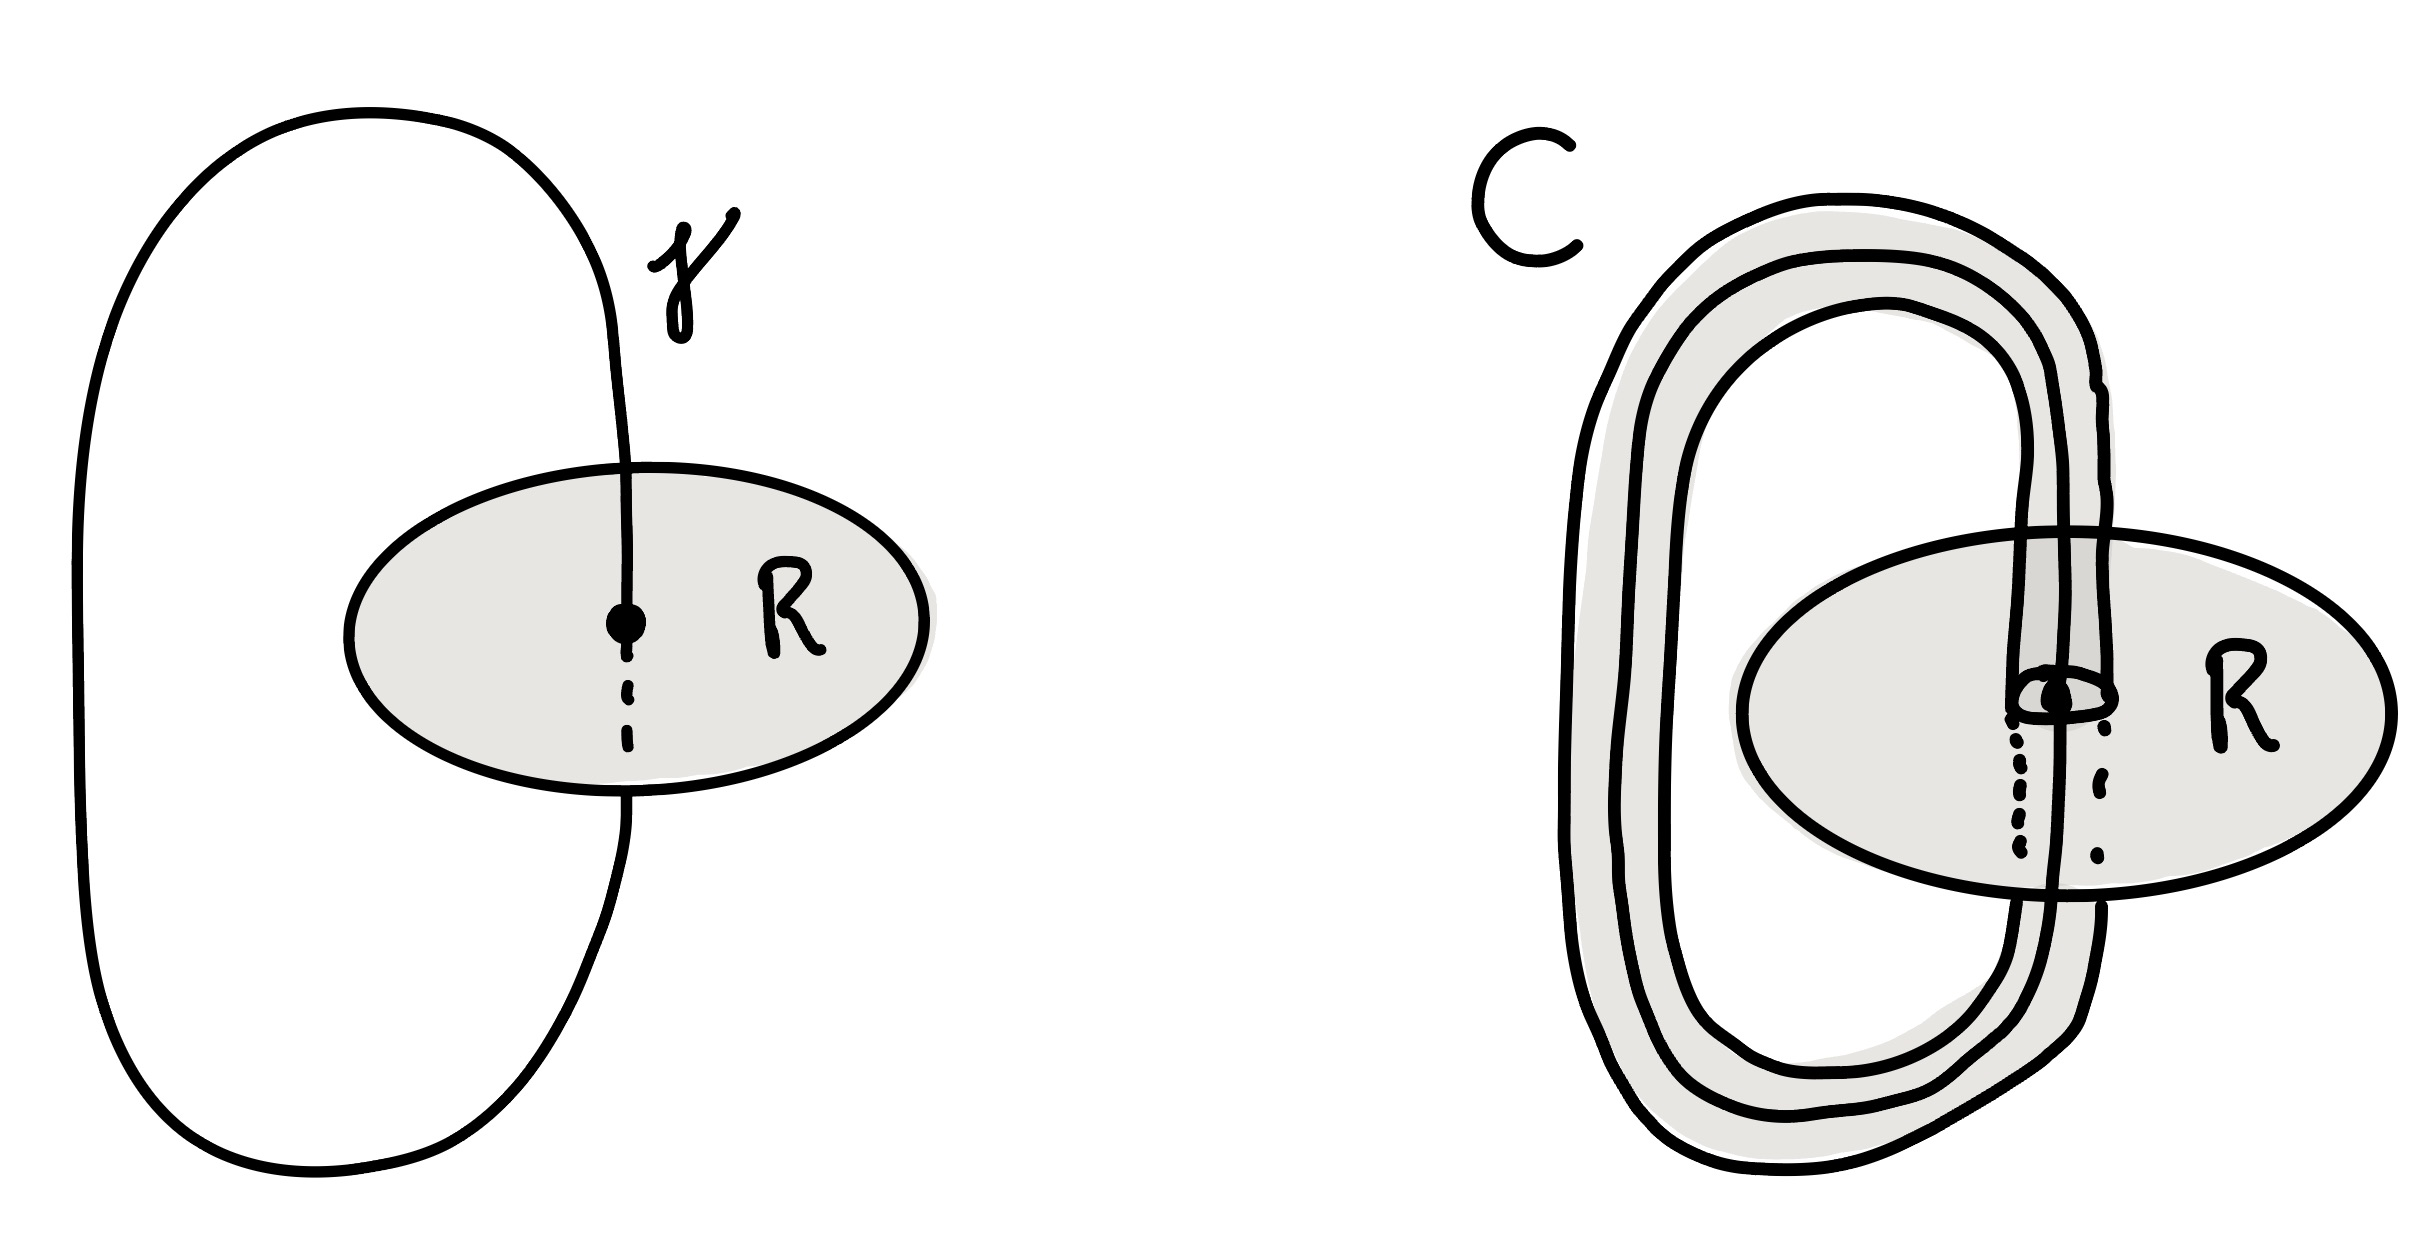
\includegraphics[width=10cm]{figures/hwk4-fig9.png}
      \captionof{figure}{Illustration of $R$, $\gamma$ and $C$.}
      \label{fig:prob1}
    \end{center}
  
  Prior to adding the vertical segments, two bounded regions $A$ and $B$ would be inaccessible. However, once they are added at the crossing points of $L$, loops can pass through.
    \begin{center}
      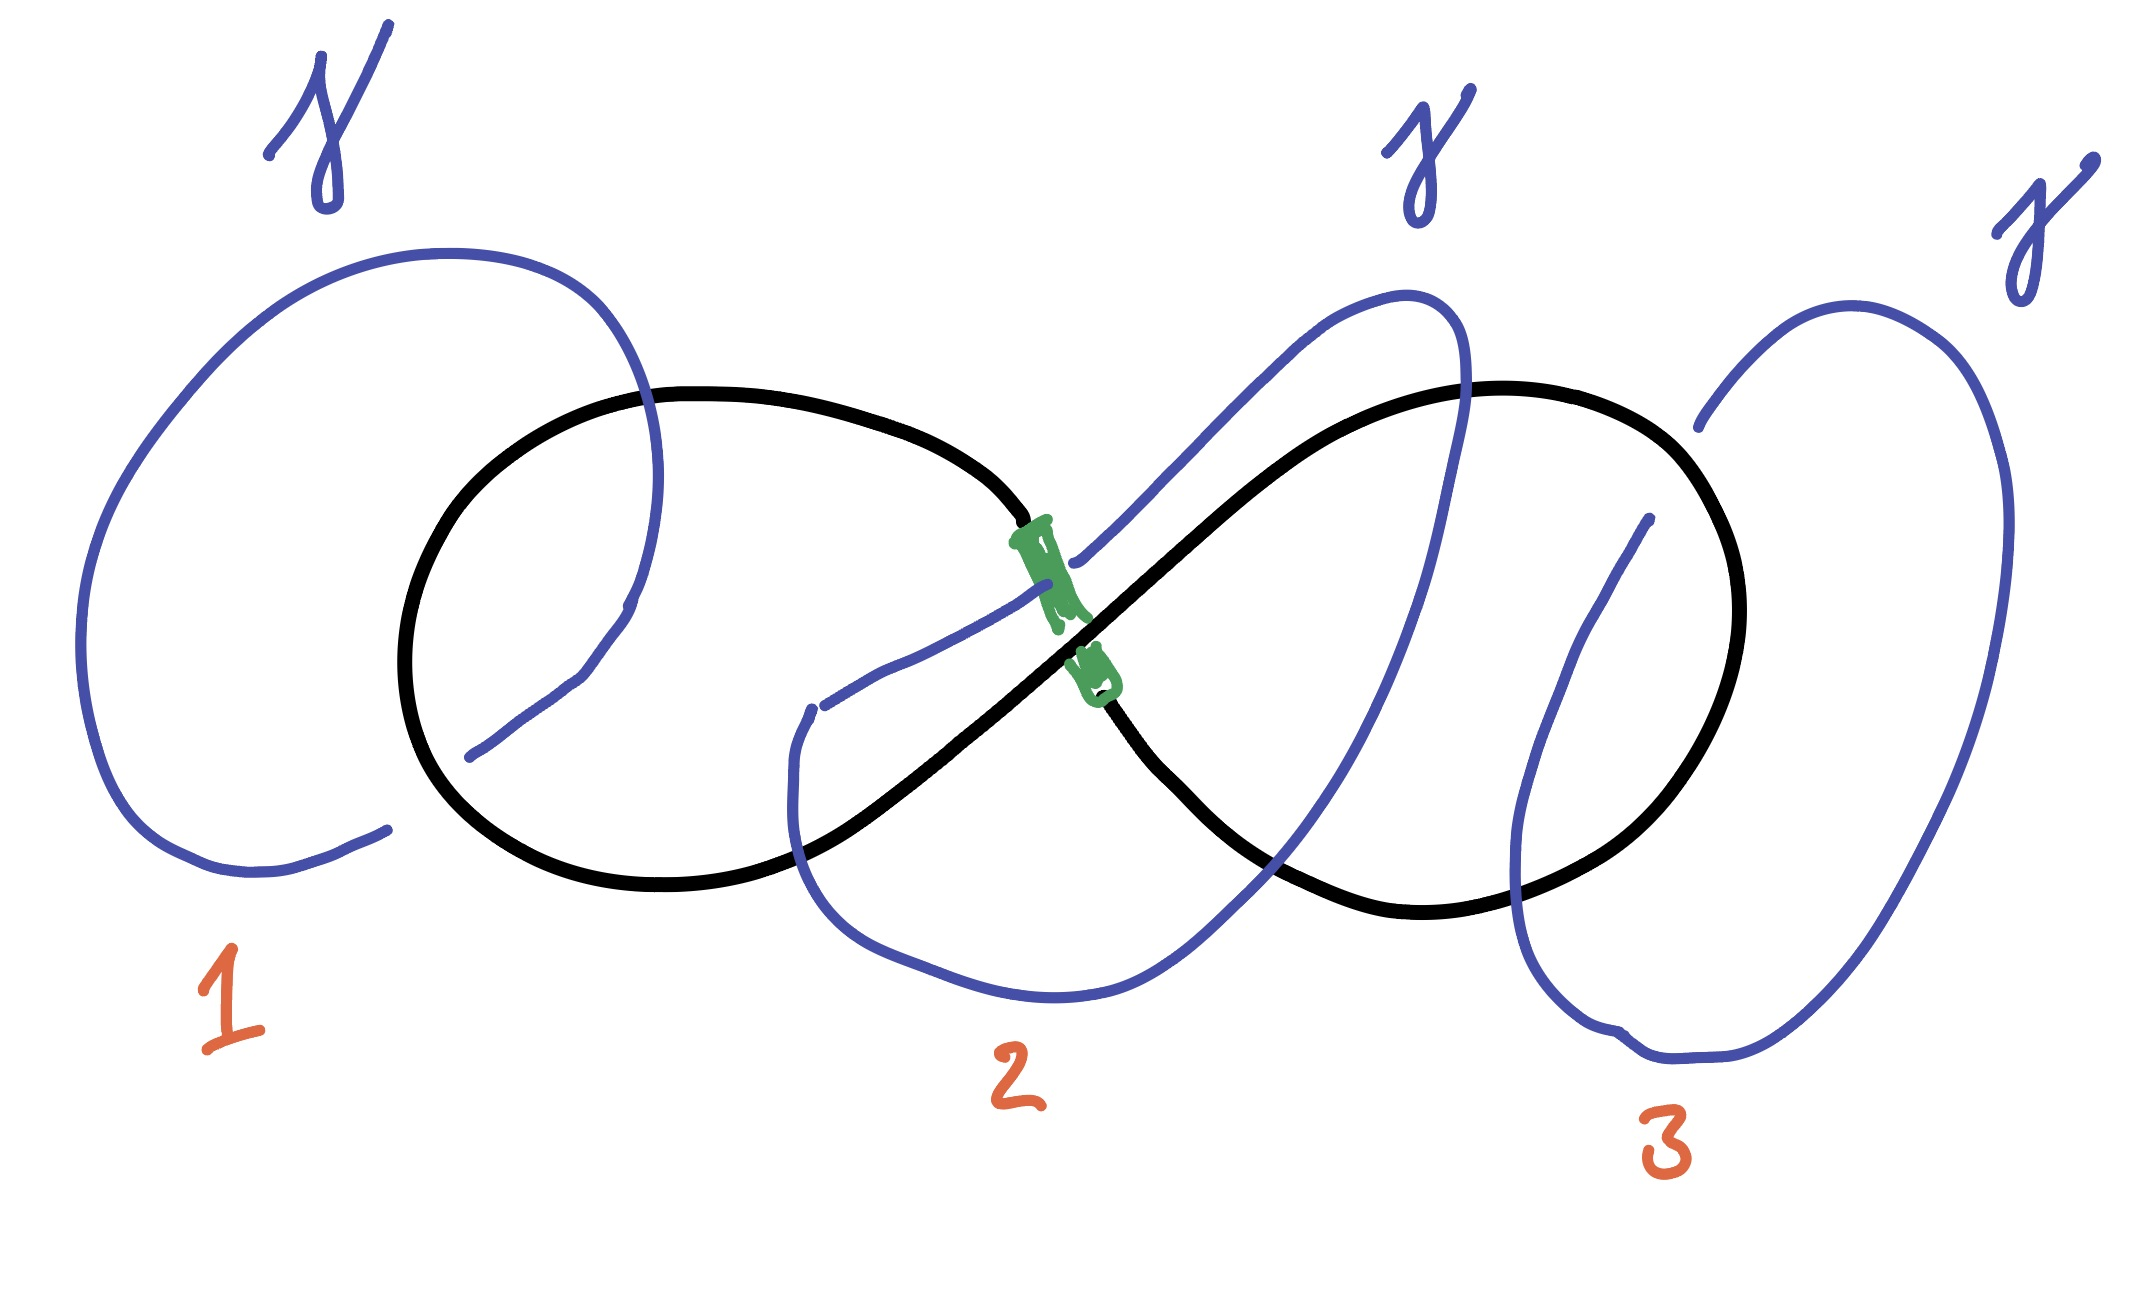
\includegraphics[width=10cm]{figures/hwk4-fig10.png}
      \captionof{figure}{Loop passing to a new bounded region through a vertical segment}
      \label{fig:prob1.1}
    \end{center}
  In the example above, passing $\gamma$ from one region to the next reverses the direction, so we get a relation $a = b^{-1}$ where $a$ and $b$ are generators corresponding to the regions in question. In a general crossing, we pass through four regions, and hence have $ab^{-1} = dc^{-1}$. This is precisely the relation used in the Dehn presentation, and hence completes the problem.
\end{prf}
\end{homework}
\end{document}
